\documentclass[openany]{book}
\usepackage[utf8]{inputenc}
\usepackage{verbatim}
\usepackage[hypertexnames=false]{hyperref}
\usepackage{amstext} 
\usepackage{array}   
% \usepackage{nath}
\newcolumntype{C}{>{$}c<{$}} 


%%%%%%%%%%%%%%%%%%%%%%%

%%%%%%%%%%%%%%%%%%%%%%%
% HOLA PACO
% ESTE ES EL ARCHIVO DE LAS DEFINICIONES ESTRUCTURALES
% VERSION 1.1 NOMÁS
%
% AUTOR ORIGINAL:
% EDUARDO (CHITO) BELMONTE GUILLAMÓN
%
% ESTE ARCHIVO ES COMUNISTA, PUEDES COMPARTIRLO SI QUIERES
%%%%%%%%%%%%%%%%%%%%%%%

%----------------------------------
%     PAQUETICOS QUE SE USAN
%----------------------------------

%--------------------------
%    PARA USAR INKSCAPE
%---------------------------
\usepackage{import}
\usepackage{hyperref}
\usepackage{xifthen}
\usepackage{pdfpages}
\usepackage{transparent}

\newcommand{\incfig}[1]{%
    \def\svgwidth{\columnwidth}
    \import{./figures/}{#1.pdf_tex}
}

\newcommand{\custincfig}[2]{%
    \def\svgwidth{#1}
    \import{./figures/}{#2.pdf_tex}
}
\newcommand{\textnexttofig}[3]{
  \begin{minipage}[l]{0.45\textwidth}
    \custincfig{#1}{#2}
  \end{minipage}
  \begin{minipage}[l]{0.45\textwidth}
    #3
  \end{minipage}
}

%%%%%%%%% FIN DEL INKSCAPE

\usepackage{parskip} % Pa parrafos wapos
\setlength{\parindent}{0.5cm} % Pa la sangría
\usepackage{graphicx} % Pa meter las imágenes
\graphicspath{{Images/}} % La ruta a las imágenes

\usepackage{tikz} % Pa dibujar cosichuelas guapas

\usepackage[spanish]{babel} % PA QUE ESTÉ EN ESPAÑOL NOMÁS

\usepackage{enumitem} % Para personalizar las LISTAS YEAH

\setlist{nolistsep} % Pa que las listas estén junticas

\usepackage{booktabs} % Esta sirve para hacer tablas fancy con multicolumns y tal pero no tengo ni puta idea de usarla

\usepackage{xcolor} % PA DEFINIR LOS COLORINES
\definecolor{turquoise}{RGB}{21,103,112} % Es un turquesica así formal
\definecolor{violet}{RGB}{ 110, 6, 187 } % Color maricón

%-------------------------------------------------
%     MÁRGENES
%-------------------------------------------------

\usepackage{geometry}
\geometry{
    top=3cm,
    bottom=3cm,
    left=3cm,
    right=3cm,
    headheight=14pt,
	footskip=1.4cm,
	headsep=10pt,
}

\usepackage{avant} % Esto es una fuente para encabezados

%\usepackage{mathptmx} % Usar simbolitos matemáticos chulos

\usepackage{microtype} % Para fuentes de maricones

\usepackage[utf8]{inputenc} % Pa los acentos

\usepackage[T1]{fontenc}

%-------------------------------------------------
% Bibliografía e índice
%-------------------------------------------------

\usepackage{makeidx} % Pa hacer un índice
\makeindex

\usepackage{titletoc}   % Para manipular la tabla de contenidos

\contentsmargin{0cm}    % Para eliminar el margen por defecto

\usepackage{titlesec} % Pa cambiar los titulos skere

\titleformat
{\chapter} % command
[display] % shape
{\centering\bfseries\Huge\normalfont} % format
{\color{turquoise}  {\normalsize\MakeUppercase{Capítulo} \thechapter }} % label
{-0.5cm} % sep
{
    \color{turquoise}
    \rule{\textwidth}{3pt}
    \vspace{1ex}
    \centering
    \setcounter{ex}{0}
    \setcounter{dummy}{0}
} % before-code
[
\vspace{-0.5cm}%
\rule{\textwidth}{3pt}
] % after-code


\titleformat{\part}
[display]
{\centering\bfseries\Huge\normalfont}
{\color{turquoise} {\normalsize \MakeUppercase{Asignatura}}}
{0pt}
{\color{turquoise}
\vspace{-0.6cm}
\rule{\textwidth}{3pt}
\vspace{1ex}
\setcounter{chapter}{0}
\setcounter{section}{0}
\setcounter{dummy}{0}
\centering
}


\titleformat{\section}
{\normalfont\Large\bfseries}{\color{turquoise}\thesection\ - }{0.5em}{}

\usepackage{fancyhdr}   % Necesario para el encabezado y el pie de página

\pagestyle{fancy}   %Para modificar los encabezados
\fancyhf{}          %Para eliminar los encabezados y pies de página por defecto.
\fancyhead[LE,RO]{\sffamily\normalsize\thepage}
\fancyfoot[C]{Ampliación de Probabilidad}
%HACER

\usepackage{amsmath,amsfonts,amssymb,amsthm,cancel} % PARA LAS MATES

%   LINEA 199, HACER CAPULLADAS

\newtheoremstyle{turquoisebox}
{0pt} %Espacio encima
{0pt} %Espacio abajo
{\normalfont} % Fuente del cuerpo
{} % Cantidad de identado
{\small\ssfamily\color{turquoise}} % Fuente en la que pone "TEOREMA"
{:} % Puntuación tras el teorema
{0.25em} %Espacio tras el teorema
{\thmname{#1}\thmnumber{#2}} %No sé si esto funciona


\newcounter{dummy}
\newcounter{ex}
\newtheorem{teoremote}[dummy]{\color{turquoise}Teorema}
\newtheorem{propositiont}{\color{turquoise}Proposición}[section]
\newtheorem{lemmat}{\color{turquoise}Lema}[section]
\newtheorem{definitionT}{\color{turquoise}Definición}[section]
\newtheorem{exerciseT}[ex]{Ejercicio}
\newtheorem{examplote}[ex]{\color{turquoise}Ejemplo}
\newtheorem{methodT}[dummy]{\color{turquoise}Método}


\RequirePackage[framemethod=default]{mdframed} % Required for creating the theorem, definition, exercise and corollary boxes

%Caja de teoremas

\newmdenv[skipabove=7pt,
skipbelow=7pt,
backgroundcolor=black!5,
linecolor=turquoise,
innerleftmargin=5pt,
innerrightmargin=5pt,
innertopmargin=5pt,
leftmargin=0cm,
rightmargin=0cm,
linewidth=3pt,
innerbottommargin=5pt]{tBox}

\newmdenv[skipabove=7pt,
skipbelow=7pt,
backgroundcolor=black!5,
linecolor=turquoise,
innerleftmargin=5pt,
innerrightmargin=5pt,
innertopmargin=5pt,
leftmargin=0cm,
rightmargin=0cm,
linewidth=1pt,
innerbottommargin=5pt]{pBox}

\newmdenv[skipabove=7pt,
skipbelow=7pt,
backgroundcolor=violet!7,
linecolor=turquoise,
innerleftmargin=5pt,
innerrightmargin=5pt,
innertopmargin=5pt,
leftmargin=0cm,
rightmargin=0cm,
rightline=false,
topline=false,
bottomline=false,
linewidth=4pt,
innerbottommargin=5pt]{mBox}

\newmdenv[skipabove=7pt,
skipbelow=7pt,
rightline=false,
leftline=true,
topline=false,
bottomline=false,
linecolor=turquoise,
innerleftmargin=5pt,
innerrightmargin=5pt,
innertopmargin=0pt,
leftmargin=0cm,
rightmargin=0cm,
linewidth=4pt,
innerbottommargin=0pt]{dBox}

\newmdenv[skipabove=7pt,
skipbelow=7pt,
rightline=false,
leftline=true,
topline=false,
bottomline=false,
backgroundcolor=black!3,
linecolor=turquoise!50,
innerleftmargin=5pt,
innerrightmargin=5pt,
innertopmargin=0pt,
innerbottommargin=5pt,
leftmargin=0cm,
rightmargin=0cm,
linewidth=4pt]{eBox}

\newmdenv[skipabove=7pt,
skipbelow=7pt,
leftline=true,
topline=false,
rightline=false,
bottomline=false,
backgroundcolor=cyan!5,
linecolor=turquoise,
innerleftmargin=5pt,
innerrightmargin=5pt,
innertopmargin=0pt,
innerbottommargin=5pt,
leftmargin=0cm,
rightmargin=0cm,
linewidth=4pt]{exBox}

\newenvironment{theorem}{\begin{tBox}\begin{teoremote}}{\end{teoremote}\end{tBox}}
\newenvironment{proposition}{\begin{pBox}\begin{propositiont}}{\end{propositiont}\end{pBox}}
\newenvironment{lemma}{\begin{pBox}\begin{lemmat}}{\end{lemmat}\end{pBox}}
\newenvironment{method}{\begin{mBox}\begin{methodT}}{\end{methodT}\end{mBox}}
\newenvironment{definition}{\begin{dBox}\begin{definitionT}}{\end{definitionT}\end{dBox}}
\newenvironment{exercise}{\begin{eBox}\begin{exerciseT}}{\hfill{\color{black}}\end{exerciseT}\end{eBox}}
\newenvironment{example}{\begin{exBox}\begin{examplote}}{\end{examplote}\end{exBox}}
\newenvironment{demonstration}{\begin{flushright}
      \color{turquoise} \textbf{Demostración}
\end{flushright}
}{\begin{flushright}
  $\square$
\end{flushright}}

\usepackage{geometry}
\geometry{
    top=3cm,
    bottom=3cm,
    left=3cm,
    right=3cm,
    headheight=14pt, 
    footskip=1.4cm,
    headsep=10pt,
}
\usepackage{graphicx}
\title{Ejercicios de Ampliación de Probabilidad}
\author{Paco Mora Caselles}
\date{\today}

\begin{document}

\maketitle

\chapter{Relación 1}
\begin{exercise}
    $$  C = \{(x,y) \in \mathbb{R} ^2 \ :\ 0<x<1,\ 0<y<1,\ y < (1-x)^2\} $$

    \begin{center}
        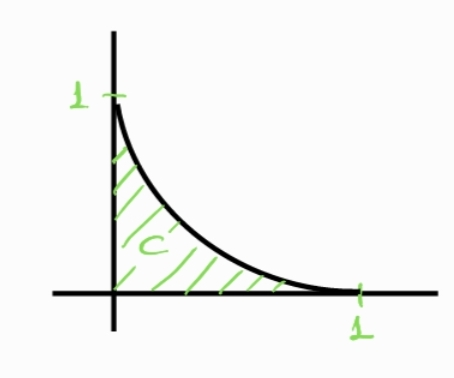
\includegraphics[scale=0.5]{1-1.jpg}
    \end{center}

    Dejamos por ahora $ f $ en función de $ k $, más tarde calculamos su valor:

    $$ f(x,y) = \left\{
    \begin{array}{lr}
        k & (x,y) \in C\\
        0 & (x,y) \not \in C   
    \end{array}
    \right. $$

    Para $ x \in (0,1) $:
    $$ f_{1}(x) = \int\limits_{}^{}f(x,y) dy = \int\limits_{0}^{(1-x)^2}k dy = k(1-x)^2 $$

    Entonces tenemos:

    $$ f_{1}(x) = \left\{
    \begin{array}{lr}
        k(1-x)^2 & x \in (0,1)\\
        0 & x \not \in (0,1)
    \end{array}
    \right. $$

    Pasamos ahora a $ f_{2}(y) $, cuando $ y \in (0,1) $:
    $$ f_{2}(y) = \int\limits_{}^{}f(x,y)dx = \int\limits_{0}^{1-y^{1/2}} = k (1-y)^{1/2} $$

    $$ f_{2}(y) = \left\{
    \begin{array}{lr}
        k(1-\sqrt{y}) & y \in (0,1) \\
        0 & y \not \in (0,1)
    \end{array}
    \right. $$

    Calculamos ahora $ E(X^{n}(1-X)^{m}) $ usamos $ f_{1}(x) $:
    $$ E(X^{n}(1-X)^{m}) = \int\limits_{}^{}x^{n}(1-x)^{m}f_{1}(x)dx = \int\limits_{0}^{1} x^{n}(1-x)^{m} k (1-x)^2 dx = k \int\limits_{0}^{1}x^{n}(1-x)^{m+2} =$$
    $$ =  kB(n+1,m+3) = k \dfrac{\Gamma(n+1)\Gamma(m+3)}{\Gamma(n+m+4)} = k \dfrac{n!(m+2)!}{(n+m+3)!} $$
    
    Los momentos de orden $ n $ respecto del origen, la esperanza y la varianza de $ X $ las podemos calcular con esta expresión. Para los primeros casos tomamos $ m=0 $ y para la varianza podemos usar que $ Var(X) = E(X^2)-E(X)^2 $

    $$ k = 3 \hspace{10mm} E(X) = \dfrac{1}{4}\hspace{10mm} E(X^2) = \dfrac{1}{10} \hspace{10mm} Var(X) = \dfrac{3}{80} $$
    
    Calculamos $ f_{2|1}(y|x) $, si $ x \in (0,1) $:
    $$ f_{2|1}(y|x) = \dfrac{f(x,y)}{f_{1}(x)} = \left\{
    \begin{array}{lr}
        \dfrac{3}{3(1-x)^2} = \dfrac{1}{(1-x)^2} & y \in (0,(1-x)^2)\\
        0 & y \not \in (0,(1-x)^2)
    \end{array}
    \right. $$

    Podemos calcular ahora $ f_{2|1}(y|x=1/2) $:
    $$ f_{2|1}(y|1/2) = \left\{
    \begin{array}{lr}
        4 & y \in (0,\dfrac{1}{4}) \\\\
        0 & y \not \in (0,\dfrac{1}{4})
    \end{array}
    \right. $$

    Para calcular $ F\left(\dfrac{1}{4},\dfrac{9}{16}\right) $ nos apoyamos en la figura para saber que basta con calcular el área del rectángulo y multiplicar por $ k $:
    
    \begin{center}
        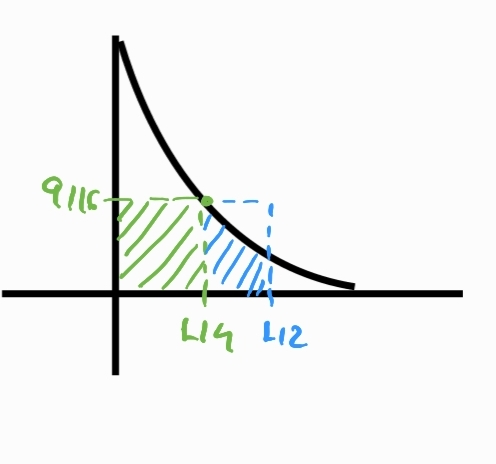
\includegraphics[scale=0.4]{1-1-2.jpg}
    \end{center}
    

    $$ F\left(\dfrac{1}{4},\dfrac{9}{16}\right) = 3 \dfrac{1}{4}\cdot \dfrac{9}{16} = \dfrac{3^3}{2^{6}}$$

    Para $ F\left(\dfrac{1}{2},\dfrac{9}{16}\right) = F\left(\dfrac{1}{4},\dfrac{9}{16}\right)+3\cdot Area\ T $, siendo $ T $ la intersección con $ C $. Sabemos entonces que:
    $$ \int\limits_{1/4}^{1/2}(1-x)^2dx = \int\limits_{1/4}^{1/2}(x^2-2x+1)dx = \dfrac{x^3}{3}-x^2+x \Biggr|_{1/4}^{1/2} = \dfrac{19}{2^{6}3} $$
    $$ F\left(\dfrac{1}{2},\dfrac{9}{16}\right) = \dfrac{3^3}{2^{6}} + 3 \dfrac{19}{2 ^{6}3} = \dfrac{23}{32} $$

    Tenemos que calcular ahora la recta de regresión de $ Y $ respecto de $ X $:
    $$ y - \mu_{y} = \dfrac{\sigma _{xy}}{\sigma_{x}^2}(x-\mu_{x}) $$
    $$ \mu_{y} = E(Y) = \int\limits_{0}^{1} y 3(1-y^{1/2})dy = 3 \int\limits_{0}^{1}(y-y^{3/2}) = \dfrac{3}{10} $$
    $$ E(XY) = \int\limits_{0}^{1} \int\limits_{0}^{(1-x)^2} 3xy dy dx = 3 \int\limits_{0}^{1} x \left[\dfrac{y^2}{2}\right]_{0} ^{(1-x)^2} d = \dfrac{3}{2} \int\limits_{0}^{1}x(1-x)^{4}dx = $$
    $$ = B(2,5) = \dfrac{3}{2} \dfrac{\Gamma(2)\Gamma(5)}{\Gamma(7)}= \dfrac{3}{2} \dfrac{1!4!}{6!} = \dfrac{1}{20} $$
    Recordemos que $ \mu_{X} = E(X) = \dfrac{1}{4} $, entonces:
    $$ \sigma_{XY}Cov(X,Y) = \dfrac{1}{2^2\cdot 5} -\dfrac{1}{2^2}\cdot \dfrac{3}{2\cdot 5} = \dfrac{2-3}{2^3\cdot 5} = -\dfrac{1}{2^3\cdot 5}$$

    Podemos expresar ya la recta de regresión (recordando que $ \sigma_{X}  = \dfrac{3}{80}$):
    $$ y-\dfrac{3}{10} = \dfrac{-1/(5\cdot 2^3)}{3/(2^{4}\cdot 5)}(x-\dfrac{1}{4}) $$
    $$ y = -\dfrac{2}{3}x+\dfrac{7}{15} $$

    Calculamos ahora $ E(Y|X=x) = m_{2|1}(x) $:
    $$ E(Y|X=x) = \int\limits_{}^{}y f_{2|1}(y|x)dy = \int\limits_{0}^{(1-x)^2}y \dfrac{1}{(1-x)^2}dy = $$
    $$ =\dfrac{1}{(1-x)^2} \dfrac{y^2}{2} \Biggr|_{0}^{(1-x)^2} = \dfrac{1}{(1-x)^2} \dfrac{(1-x)^{4}}{2} = \dfrac{(1-x)^2}{2} $$


\end{exercise}


\begin{exercise}
    $$ E(X) = 2,\ Var(X) = 3\ X\ \text{simétrica} $$
    
    $$ \alpha_{3} = E(X^3) = E((X-2+2)^3) = E((X-2)^3+3(X-2)^22+3(X-2)2^2+2^3) = $$
    $$= E((X-2)^3)+6E((X-2)^2) +12 E(X-2)+E(2^3) = 0 + 6 Var(X)+0+2^3 = 6\cdot 3+8 = 26$$
\end{exercise}


\begin{exercise}
    $  $\\
    El número de de posibilidades totales es claramente $ \binom{N}{n} $, la distribución de probabilidad es entonces:

    $$ P(X_1=r_1,X_2=r_2,X_3=r_3) = \dfrac{\binom{n_1}{r_1}\binom{n_2}{r_2}\binom{n_3}{r_3}}{\binom{N}{n}} $$
    Claramente necesitamos $ n\leq N,\ r_1+r_2+r_3=n $

    Calculamos ahora $ \alpha_{(3)} $:
    $$ E(X_1 ^{(3)}) = E(X_1(X_1-1)(X_1-2)) = \sum\limits_{r_1+r_2+r_3=n}^{}r_1(r_1-1)(r_1-2)\dfrac{\binom{n_1}{r_1}\binom{n_2}{r_2}\binom{n_3}{r_3}}{\binom{N}{n}} $$

    Nos fijamos que:

    $$r_1(r_1-1)(r_1-2)  \binom{N_1}{r_1} = r_1(r_1-1)(r_1-2) \dfrac{N_1 ^{(r_1)}}{r_1(r_1-1)(r_1-2)\cdots 2\cdot 1} = $$
    $$ =\dfrac{N_1 ^{(r_1)}}{(r_1-3)!} = N_1(N_1-1)(N_1-2) \dfrac{(N_1-3) ^{(r_1-3)}}{(r_1-3)!}  = N_1(N_1-1)(N_1-2)\binom{N_1-3}{r_1-3}$$

    Entonces volviendo a la igualdad anterior:
    $$ P(X_1=r_1) = \sum\limits_{r_1+r_2+r_3=n}^{}N_1(N_1-1)(N_1-2) \dfrac{\binom{N_1-3}{r_1-3}\binom{N_2}{r_2}\binom{N_3}{r_3}}{\binom{N}{n}} =  $$
    $$ N_1(N_1-1)(N_1-2)\sum\limits_{r_1+r_2+r_3=n}^{} \dfrac{\binom{N_1-3}{r_1-3}\binom{N_2}{r_2}\binom{N_3}{r_3}}{\binom{N}{n}} = N_1(N_1-1)(N_1-2) \dfrac{\binom{N-3}{n-3}}{\binom{N}{n}} =$$
    $$ = N_1(N_1-1)(N_2-2) \dfrac{(N-3) ^{(n-3)}n!}{(n-3)!N ^{(n)}} = \dfrac{N_1 ^{(3)}n ^{(3)}}{N ^{(3)}} $$
\end{exercise}


\begin{exercise}
    $  $
    \begin{flushright}
        \textbf{Apartado a)}
    \end{flushright}

    Observemos primero que no hay dos pares de la forma $ (a,b),\ (a,c) $ de forma que ambos tengan probabilidad no nula. Igual forma, no hay pares $ (b,a),\ (c,a) $ tales que se tomen ambos valores con probabilidad no nula. Por tanto, para ver la distribución marginal de $ X $ podemos omitir los valores que toma $ Y $:
    $$ P(X=0) = P(X=1) = P(X=2) = \dfrac{1}{3} $$

    De forma análoga para la v.a. $ Y $: 
    $$ P(Y=1) = P(Y=2) = P(Y=3) = \dfrac{1}{3} $$

    Las esperanzas entonces de estas vvaa son:
    $$ E(X) = (0+1+2)\cdot \dfrac{1}{3} = 1 $$
    $$ E(Y) = (1+2+3)\cdot \dfrac{1}{3} = 2 $$

    Hacemos también los cálculos necesarios para hacer la recta de regresión:
    $$ E(XY) = (0\cdot 1+1\cdot 2+2\cdot 3) \dfrac{1}{3} = \dfrac{8}{3} $$
    $$ Cov(X,Y) = E(XY) - E(X)E(Y) = \dfrac{8}{3}*2 =\dfrac{2}{3} $$
    $$ E(X^2) = (0+1+4)\dfrac{1}{3} = \dfrac{5}{3} $$
    $$ Var(X) = E(X^2)-E(X)^2 = \dfrac{5}{3}-1 = \dfrac{2}{3} $$

    La recta de regresión de $ Y $ sobre $ X $ es entonces:
    $$ y-2 = \dfrac{\dfrac{2}{3}}{\dfrac{2}{3}}(x-1) \implies y -2 = x-1 \implies y = x+1 $$

    Calculamos ahora el coeficiente de correlación para poder ver $ Var(Y-X^{*}) $:
    $$ \rho = \dfrac{\sigma_{XY}}{\sigma_{X}\sigma_{Y}} = \dfrac{\dfrac{2}{3}}{\sqrt{\dfrac{2}{3}}\sqrt{\dfrac{2}{3}}} = 1 $$

    Este valor de $ \rho $ nos indica que $ X $ y $ Y $ son dependientes linealmente. Calculamos ahora $ Var(Y-X^*) $

    $$ Var(Y-X^*) = \sigma_{Y}^2(1-\rho ^2) = 0 $$

    \begin{flushright}
        \textbf{Apartado b)}
    \end{flushright}

    Para calcular las $ vvaa $ marginales solo tenemos que sumar los elementos de la misma fila o columna. Por ejemplo:

    $$ P(X=0) = \dfrac{1}{3}+\dfrac{1}{6}+\dfrac{1}{9} = \dfrac{11}{18} $$

    Obtenemos así:
    $$ P(X=0) = \dfrac{11}{18} \hspace{5mm} P(X=1) = \dfrac{5}{18} \hspace{5mm} P(X=2) = \dfrac{2}{18}$$
    $$ P(Y=0) = \dfrac{11}{18} \hspace{5mm} P(Y=1) = \dfrac{5}{18} \hspace{5mm} P(Y=2) = \dfrac{2}{18} $$

    También podemos obtener $ E(X) = E(Y) = \dfrac{1}{2} $, $ Var(X),Var(Y) = \dfrac{17}{36} $ y $ Cov(X,Y) = -\dfrac{5}{36} $.

    Entonces la recta de regresión de $ X $ sobre $ Y $ es:
    $$ Y-\mu_{Y} = \dfrac{\sigma_{XY}}{\sigma_{X}^2}(x-\mu_{X}) $$
    $$ y-\dfrac{1}{2} = \dfrac{-\dfrac{5}{36}}{\dfrac{17}{36}} \left(x-\dfrac{1}{2}\right) $$
    $$ y = -\dfrac{5}{17}x+\dfrac{11}{17} $$
    
    Como las esperanzas y las varianzas son iguales, obtenemos que el cálculo de la recta de regresión de $ Y $ sobre $ X $ es igual:
    $$ x = -\dfrac{5}{17}y+\dfrac{11}{17} $$

    Calcularemos ahora $ Var(Y-X^*) $:
    $$ Var(Y-X^* ) = \sigma_{Y}^2 (1-\rho ^2) = \dfrac{17}{36} \left( 1-\dfrac{25/36^2}{17^2/36} \right) = \dfrac{17}{36} \left( \dfrac{17^2-25}{17^2}\right) = \dfrac{11}{3\cdot 17}  $$

    Para la varianza residual de $ X $ sobre $ Y $, vemos que es igual porque coinciden sus esperanzas y sus varianzas.


\end{exercise}


\chapter{Relación 2}

\begin{exercise}
    $  $\\ 
    Vemos en primer lugar cómo es el recinto del ejercicio:
    \begin{center}
        \includegraphics*[scale=0.5]{2-1-1.jpg}
        
    \end{center}
    
    $$ \alpha_{n.m} = E(X^{n}Y^{m}) = \int\limits_{}^{}x^{n}y^{m} \cdot  \dfrac{1}{y} = \int\limits_{0}^{1}\int\limits_{0}^{y}  = x^{n}x^{m-1}dxdy  = $$ 
    $$= \int\limits_{0}^{1} y ^{m-1} \left( \dfrac{x^{n+1}}{n+1} \right) \Biggr|_{0}^{y} dy = \dfrac{1}{n+1} \int\limits_{0}^{1} y^{m-1}y^{n+1}dy = \dfrac{1}{n+1} \dfrac{1}{m+n+1} $$

    Con este resultado podemos obtener los valores:
    $$ E(Y) = \dfrac{1}{2} \hspace{5mm} E(Y^3) = \dfrac{1}{3} \hspace{5mm} E(XY) = \dfrac{1}{6} \hspace{5mm} E(X) = \dfrac{1}{4} $$
    
    Entonces tenemos que $ Var(Y) = \dfrac{1}{3}-\dfrac{1}{4} = \dfrac{1}{12} $ y $ Cov(X,Y) = \dfrac{1}{6}-\dfrac{1}{4}\cdot \dfrac{1}{2} = \dfrac{1}{24} $

    Para calcular la recta de regresión obtenemos primero:
    $$ \beta_{X/Y} = \dfrac{\sigma_{XY}}{\sigma_{Y}^2} = \dfrac{1/24}{1/12} = \dfrac{1}{2} $$
    
    Y la recta de regresión que nos piden queda:
    $$ x - \dfrac{1}{4} = \dfrac{1}{2} \left( y-\dfrac{1}{2} \right) $$
    $$ x = \dfrac{1}{2}y $$

    Calcularemos ahora la curva de regresión de $ X $ sobre $ Y $:
    $$  x = m_{1|2}(y) \hspace{5mm} m_{1|2}(y) = E(X|Y=y) = \int\limits_{}^{}x f_{1|2}(x|y)dx $$

    Entonces, para los valores de $ y $ para los que $ f_{2}(y)>0 $ tendremos:
    $$ f_{1|2}(x|y) = \dfrac{f(x,y)}{f_{2}(y)} $$

    Calcularemos ahora $ f_{2}(y) $:

    $$\text{Si $ y \in (0,1)$: }  f_{2}(y) = \int\limits_{}^{}f(x,y)dx = \int\limits_{0}^{y} \dfrac{1}{y}dx = \dfrac{1}{y}x \Biggr|_{0}^{1} = 1 $$


    $$ f_{2}(y) = I_{(0,1)}(y) $$

    Volvemos ahora al cálculo de $ f_{1|2}(x|y) $. Dado $ y \in (0,1) $:
    $$ f_{1|2}(x|y) = \dfrac{1/y}{1} = \dfrac{1}{y} \hspace{5mm} x \in (0,y) $$
    $$ f_{1|2}(x|y) = 0 \hspace{5mm} x \not  \in (0,y) $$

    Podemos calcular ahora $ m_{1|2}(y) $:
    $$ E(X|Y=y) = \int\limits_{0}^{y}x \dfrac{1}{y} dx = \dfrac{1}{y}\dfrac{x^2}{2} \Biggr|_{0}^{y} = \dfrac{y}{2} $$

    Entonces la curva de regresión es $ x = \dfrac{y}{2} $. Notemos que es una recta, en este caso \textbf{necesariamente coincidirá con la recta de regresión}. Entonces, si hubiéramos calculado primero la curva de regresión, no tendríamos que calcular la recta porque sabemos que coincidiría.

    
\end{exercise}

\setcounter{ex}{1}

\begin{exercise}
    $$ f(t_1,t_2,t_3,t_4) = \dfrac{1}{4}(t_1+t_2+t_3+t_1t_2t_3) = E(t_1^{X_1}t_2^{X_2}t_3^{X_3}) = \sum\limits_{}^{}p_{i_1i_2i_3}t_1^{i_1}t_2^{i_2}t_3^{i_3} $$

    De este último término, en cada sumando, $ p_{i_1i_2i_3} $ representa $ P(X_1=i_1,X_2=i_2,X_3=i_3) $

    Viendo el valor de $ f $, sabemos que la vvaa $ (X_1,X_2,X_3) $ toma los valores $ (1,0,0),(0,1,0),$  $(0,0,1),(1,1,1) $ con probabilidad de $ \dfrac{1}{4} $ en cada una de ellas.

    Vamos a comprobar si $ X_1,X_2 $ son independientes. Para ello, vemos si $ f_{12}(t_1,t_2) = f_{1}(t_1) \cdot f_{2}(t_2) $. Estas funciones no las conocemos, pero como sabemos que $ f $ se puede representar como $ E(t_1^{X_1}t_2^{X_2}t_3^{X_3}) $, si hacemos $ t_3=1 $:
    $$ f_{12}(t_1,t_2) = E(t_1^{X_1},t_2^{X_2}) = E(t_1^{X_1}t_2^{X_2}1^{X_3}) = \dfrac{1}{4}(t_1+t_2+1+t_1t_2) $$
    
    De igual forma podemos hacer:
    $$ f_{1}(t_1) = E(t_1^{X_1}) = E(t_1^{X_1}1^{X_2}1^{X_3}) = \dfrac{1}{4}(t_1+1+1+t_1) = \dfrac{1+t_1}{2} $$
    $$ f_{2}(t_2) = \dfrac{1+t_2}{2} $$

    Para comprobar la independencia solo tenemos que ver si $ f_{12} = f_{1}f_{2} $:
    $$f_{1}f_{2} = \dfrac{1}{2}(1+t_1) \cdot \dfrac{1}{2}(1+t_2) = \dfrac{1}{4}(t_1+t_2+1+t_1t_2) = f_{12} $$

    Luego $ X_1,X_2 $ son independientes y de forma análoga: $ X_2,X_3 $ son independientes y $ X_2,X_3 $ son independientes. Es decir, son independientes dos a dos.
    
    Para comprobar que son independientes, tendremos que ver si $ f(t_1,t_2,t_3) = f_{1}(t_1) \cdot f_{2}(t_2)\cdot f_{3}(t_3) $:
    $$ f_{1}f_{2}f_{3} = \dfrac{1}{2^3}(1+t_1)(1+t_2)(1+t_3) = \dfrac{1}{2^3}(1+t_1+t_2+t_1t_2)(1+t_3)= $$
    $$ = \dfrac{1}{2^3}(1+t_1+t_2+t_1t_2+t_3+t_1t_3+t_2t_3+t_1t_2t_3) \ne f(t_1,t_2,t_3) $$

    Por tanto, las vvaa no son independientes.

    Para calcular el apartado c), haremos las parciales:
    $$ \dfrac{\partial f}{\partial t_1} = \dfrac{1}{4}(t_1+t_2t_3) $$
    $$ \dfrac{\partial f}{\partial t_1}(1,1,1) = E(X_1) = \dfrac{1}{2} $$

    Por la simetría de $ f $, $ E(X_2) = E(X_3) = \dfrac{1}{2} $. Vamos ahora con las varianzas, que de nuevo bastará con calcular la de $ X_1 $:

    $$ \dfrac{\partial ^2 f}{\partial t_1^2} = E(X_1 ^{(2)}) = E(X_1^2-X_1) = 0 = E(X_1^2)-E(X_1 )\implies E(X_1^2) = \dfrac{1}{2} $$

    $$Var(X_{2}) =Var(X_3) = Var(X_1) = E(X_1^2)-E(X_1)^2 = \dfrac{1}{2}-\dfrac{1}{4}=\dfrac{1}{4} $$

    El cálculo de la covarianza es rápido, como $ X_1,X_2,X_3 $ son independientes \textbf{por parejas}, tenemos que:
    $$ Cov(X_1,X_2) = Cov(X_1,X_3) = Cov(X_2,X_3) = 0 $$

    En el caso general, es decir, si no fueran independientes:
    $$ \dfrac{\partial f}{\partial t_1 \partial t_2} = \dfrac{1}{4}t_3 $$
    $$ \dfrac{\partial f}{\partial t_1 \partial t_2}(1,1) = E(X_1X_2) = \dfrac{1}{4} $$
    $$ Cov(X_1,X_2) = E(X_1X_2)-E(X_1)E(X_2) = \dfrac{1}{4}-\dfrac{1}{4} = 0 $$

    \begin{flushright}
        \textbf{Anotación importante)}

    \end{flushright}

    Es importante notar las diferencias entre $ X+Y+Z $ y $ (X,Y,Z) $:

    Sean $ X_1,X_2,X_3 $ independientes con funciones:
    $$ f_{1}(t) = \dfrac{1}{2}(1+t) $$
    $$ f_{2}(t) = \dfrac{1}{3}(1+t+t^2) $$
    $$ f_{3}(t) = \dfrac{1}{2}(1+t) $$

    Entonces la vvaa $ Z = X_1+X_2+X_3 $ es unidimensional, y además $ f_{Z}(t) = \dfrac{1}{2}(1+t)\dfrac{1}{3}(1+t+t^2)\dfrac{1}{2}(1+t) $ \textbf{con un solo parámetro}.

    Si definimos ahora la vvaa $ X = (X_1,X_2,X_3) $, es de tres dimensiones con función generatriz:
    $$ f_{X}(t_1,t_2,t_3)= \dfrac{1}{2}(1+t_1)\dfrac{1}{3}(1+t_2+t_2^2)\dfrac{1}{2}(1+t_3)$$

\end{exercise}

\begin{exercise}
    $  $\\
    Sabemos que, para $ X,Y,Z $ tenemos:
    $$ f(x)=
    \left\{
    \begin{array}{lr}
        1 & x \in (0,1)\\
        0 & x \not \in (0,1)
    \end{array}
    \right.
    $$
    Entonces $ E(X)=E(Y)=E(Z)  $ es:
    $$ \int\limits_{0}^{1} xdx = \dfrac{x^2}{2} \Biggr|_{0}^{1} = \dfrac{1}{2} $$

    $$ E(X^2) = E(Y^2) = E(Z^2) = \int\limits_{0}^{1} x ^2 = \dfrac{s^3}{3} \Biggr|_{0}^{1} = \dfrac{1}{3}$$
    $$ Var(X)=\dfrac{1}{3}-\dfrac{1}{4} = \dfrac{1}{12} $$

    Entonces:

    $$ E(U) = a \dfrac{1}{2}+b \dfrac{1}{2} +c \dfrac{1}{2} = \dfrac{a+b+c}{2} $$
    
    Como las variables son independientes:
    $$ Var(U) = Var(aX)+Var(bY) + Var(cZ) = (a^2+b^2+c^2) = \dfrac{1}{12} $$

    Nos piden también los momentos de orden 3 y 4 respecto de la media. Utilizamos el subapartado de \textbf{Momentos de sumas}. Siguiendo un procedimiento como el de este subapartado llegamos a que solo necesitamos expresiones como $ \mu_{3}(aX) = E\left(aX-\dfrac{a}{2}\right) = 0 $ ya que estas vvaa son simétricas respecto de su media. En definitiva:
    $$ E((U-E(U))^3) = \mu_{3}(aX)+\mu_{3}(bY)+\mu_{3}(cZ) = a \mu_{3}(X) + b \mu_{3}(Y) + c\mu_{3}(Z) = 0 $$

    $$ \mu_{4}(U) = \mu_{4}(aX) + \mu_{4}(bY) + \mu_{4}(cZ) + 6(\mu_{2}(aX)\mu_{2}(bY)+\mu_{2}(aX)\mu_{2}(cZ) + \mu_{2}(bY)\mu_{2}(cZ)) $$
    
    Vamos a hacer el cálculo para un $ n $ general de:
    $$ \mu_{n}(X) = E\left( \left( X-\dfrac{1}{2}   \right)^2\right) = \int\limits_{0}^{1} \left( x-\dfrac{1}{2} \right) ^{n} dx = \dfrac{(x-1/2)^{n+1}}{n+1} \Biggr|_{0}^{1} = \dfrac{(1/2)^{n+1}}{n+1}-\dfrac{(-1/2)^{n+1}}{n+1} =$$
    $$ = \dfrac{1}{(n+1)2^{n+1}} (1+(-1)^{n}) $$

    Luego:
    $$ \mu_{4}(X) = \dfrac{1}{5\cdot 2^{4}} $$
    $$ \mu_{2}(X) = \dfrac{1}{12} \hspace{5mm} \text{(como ya habíamos calculado antes)} $$

    Volviendo ahora a $ \mu_{4}(U) $:
    $$ \mu_{4}(U) =  (a^{4}+b^{4}+c^{4})\dfrac{1}{5\cdot 2^{4}} + 6 \Big(a^2b^2+a^2c^2+b^2c^2 \Big ) \dfrac{1}{3^2 2^{4}}$$

    Calculamos ahora la función generatriz de momentos (recordemos que la función generatriz no está definida porque $ X,Y,Z $ toman valores no enteros). Usaremos la independencia de las vvaa:

    $$E(e^{tU}) = E(e^{atX})E(e^{btY}) E(e^{ctZ}) $$

    Tendremos que calcular la función generatriz de momentos de cada vvaa (son todas iguales):
    $$ E(e^{tX}) = \int\limits_{0}^{1} e^{tx} dx = \dfrac{e^{tx}}{t} \Biggr|_{0}^{1} = \dfrac{e^{t}-1}{t} $$
    
    En el caso de $ aX $ (análogamente para $ bY,cZ $):
    $$ g_{aX}(t) = E(e^{taX}) = \dfrac{e^{at}-1}{at} $$

    Entonces volviendo a la vvaa $ U $:
    $$ g_{U}(t) = \dfrac{e^{at}-1}{at}\cdot \dfrac{e^{bt}-1}{bt}\cdot \dfrac{e^{ct}-1}{ct} $$

    La función característica de $ U $ será entonces:
    $$ \varphi_{U} (t) = \dfrac{(e^{iat}-1)(e^{ibt}-1)(e^{ict}-1)}{i\cdot a\cdot b\cdot c t^3}  = \dfrac{-i(e^{iat}-1)(e^{ibt}-1)(e^{ict}-1)}{ a\cdot b\cdot c \cdot  t^3}$$

    Nos piden comprobar si es simétrica:
    $$ E(e^{itU}) = E(e^{it(aX+bY+cZ)}) = E(e^{iatX})E(e^{ibtX})E(e^{ictX}) = \dfrac{e^{iat}-1}{iat} \cdot \dfrac{e^{ibt}-1}{ibt} \cdot  \dfrac{e^{ict}-1}{ict} = $$
    $$=e^{iat/2}e^{ibt/2}e^{ict/2} 2^3 $$
    % TODO por copiar 17/2

\end{exercise}  


\begin{exercise}
    $  $ \\ 

    Para calcular $ A $:
    $$ 1 = \sum\limits_{r=0}^{+\infty} \dfrac{A}{(2r)!} = A \sum\limits_{r=0}^{+\infty}\dfrac{1}{(2r)!} = A \dfrac{1}{2} \left(\sum\limits_{k=0}^{+\infty} \dfrac{(1)^{k}}{k!}+ \sum\limits_{k=0}^{+\infty} \dfrac{(-1)^{k}}{k!} \right) = A \dfrac{1}{2} (e+e^{-1}) \implies A = \dfrac{2}{e+e ^{-1}} $$

    $ B $ se saca de forma análoga:
    $$ 1 = \sum\limits_{r=0}^{+\infty} \dfrac{B}{(2r+1)!} = B \dfrac{1}{2}\left( \sum\limits_{k=0}^{+\infty}\dfrac{1^{k}}{k!} - \sum\limits_{k=0}^{+\infty} \dfrac{(-1)^{k}}{k!} \right) = B \dfrac{1}{2}(e-e ^{-1}) \implies B = \dfrac{2}{e-e ^{-1}} $$

    Calculamos ahora las funciones generatrices:
    $$ f_{X}(t) = \sum\limits_{r=0}^{+\infty} \dfrac{A}{(2r)!} t ^{2r} = \dfrac{2}{e+e ^{-1}} \sum\limits_{r=0}^{+\infty} \dfrac{t ^{2r}}{(2r)!} = \dfrac{2}{e + e ^{-1}}\cdot (e ^{t}+e^{-t})$$

    Igualmente:
    $$ f_{Y}(t) = \dfrac{e^{t}-e^{-t}}{e-e ^{-1}} $$

    Como $ X,Y $ son independientes:
    $$ f_{Z}(t) = f_{X}(t)\cdot f_{Y}(t) = \dfrac{e^{t}+e^{-t}}{e+e ^{-1}} \cdot \dfrac{e^{t}-e^{-t}}{e-e ^{-1}} = \dfrac{e^{2t}-e^{-2t}}{e^2-e^{-2}} = $$
    $$=  \dfrac{1}{e^2-e^{-2}} \left( \sum\limits_{k=0}^{+\infty} \dfrac{(2t)^{k}}{k!} - \sum\limits_{k=0}^{+\infty} \dfrac{(-2t)^{k}}{k!} \right) = \dfrac{1}{e^2-e^{-2}} \sum\limits_{r=0}^{+\infty} \dfrac{2(2t)^{2r+1}}{(2r+1)!} = \dfrac{1}{e^2e^{-2}} \sum\limits_{r=0}^{+\infty} \dfrac{2\cdot 2^{r+1}}{(2r+1)!} t ^{2r+1}  $$

    Luego tenemos que, para $ r=0,1,2,... $:

    $$ P(Z=2r+1) = \dfrac{1}{e^2-e^{-2}} \dfrac{2\cdot 2^{2r+1}}{(2r+1)!} $$

    El último apartado lo haremos derivando la expresión sin desarrollar las exponenciales:
    $$ E(Z) = 2 \dfrac{e^2+e^{-2}}{e^2-e^{e-2}} $$
    $$ E(Z(Z-1)) = f''_{Z}(1) = 4 $$
    $$ Var(Z) = 2 \dfrac{e^{4}-8-e^{-4}}{(e^2-e^{-2})^2} $$

\end{exercise}


\begin{exercise}
    $  $
    \begin{flushright}
        \textbf{Apartado a)}
    \end{flushright}

    $$ \alpha (t) = \dfrac{1+\cos(t)+\cos(2t)}{3} $$
    
    Comprobemos que es función característica. Si conseguimos expresar $ \alpha $ de la forma $ \sum\limits_{}^{} p_n e^{itx_n} $ ($ \sum\limits_{}^{} p_n = 1  $), tendríamos que $ \alpha $ es función característica de una $ vvaa $ discreta.

    Usaremos que:
    $$ \cos(t) = \dfrac{1}{2} \left( e^{it} + e^{-it}\right)  $$
    $$ \cos(2t) = \dfrac{1}{2} \left( e^{ixt}+e^{-ixt} \right) $$

    Entonces nos queda:
    $$ \alpha(t) = \dfrac{1}{3} e^{0} +\dfrac{1}{3} \dfrac{1}{2} (e^{it}+e^{-it})+\dfrac{1}{3} \dfrac{1}{2} (e^{2it}+e^{-2it}) = $$
    $$ = \dfrac{1}{3} e^{0} +\dfrac{1}{6} e^{it}+\dfrac{1}{6}e^{-it}+\dfrac{1}{6}e^{2it}+\dfrac{1}{6}e^{-2it} $$

    Entonces todas las constantes que multiplican a exponenciales son no negativas y suman 1. Entonces $ \alpha $ es la función característica de la vvaa que toma valores $ \{0,1,-1,2,-2\} $ con probabilidades:
    $$ P(X=0) = \dfrac{1}{3}\hspace{10mm} P(X=1)=P(X=-1)=P(X=2)=P(X=-2) = \dfrac{1}{6} $$

    \begin{flushright}
        \textbf{Apartado b)}
    \end{flushright}

    $$ \alpha(t) = \dfrac{1}{1+t^3} $$
    Esta función no esta acotada en -1 por lo que no puede ser función característica.


    \begin{flushright}
        \textbf{Apartado c)}
    \end{flushright}

    $$ \alpha(t) = \dfrac{1}{1+t^4} $$

    Recordemos la relación entre la existencia de los momentos de orden $ n $ y la existencia de la derivada de orden $ n $ en el origen.
    $$ \alpha'(t) = -(1+t ^{4})^{-2}4t^3 \hspace{5mm} \alpha'(0) = 0 $$
    $$ \alpha''(t) = ... \hspace{5mm} \alpha''(0) = 0  $$
    Entonces si existe $ X $, $E(X)=0\ E(X^2) = i^2 \alpha''(0) = 0 $, entonces la varianza sería nula y la función sería constante, pero la función característica de una distribución uniforme no es $ \alpha $



\end{exercise}

\chapter{Relación 3}

\begin{exercise}
    $$ f (x,y) = k y I_{D}\hspace{5mm} D = \{(x,y) \in \mathbb{R}^2:\ 0<x<1,\ 0<y<x\} $$
    
    \begin{flushright}
        \textbf{Apartado a)}
    \end{flushright}


    Dejamos el cálculo de $ k $ para luego. Vamos con $ f_{2} $:
    $$ f_{2}(y) = \int\limits_{\mathbb{R}}^{}f(x,y)dx = \int\limits_{y}^{1} ky dx = ky(1-y)\ y \in (0,1) $$

    $$ E(Y^{m}(1-Y)^{n}) = \int\limits_{0}^{1}k y ^{m}(1-y)^{n} y (1-y)dy = kB(m+2,n+2) = k \dfrac{\Gamma(m+2)\Gamma(n+2)}{\Gamma(m+n+4)} = $$
    $$ = k \dfrac{(m+1)!(n+1!)}{(m+n+3)!} $$

    Haciendo $ n = 0 $ obtenemos $ \alpha_{r} = E(Y^{r}) $
    $$ \alpha_{r} = k \dfrac{(r+1)!}{(r+3)!} = \dfrac{k}{(r+3)(r+2)} $$

    Para obtener el valor de $ k $ podemos haciendo $ m = n = 0 $:
    $$ m = n = 0 \implies \int\limits_{0}^{1} f_{2}(y)dy = k \dfrac{1}{3!} = \dfrac{k}{6} = 1 \implies k = 6 $$

    Como $ Y $ es acotada entre 0 y 1, $ E(e^{aY}) = E(e^{-aY}) $ son finitos, con lo que podemos expresar $ g(t) $ como la siguiente serie que será convergente:
    $$ g(t) = 6\sum\limits_{r=0}^{+\infty} \dfrac{1}{(r+3)(r+2)r!} t ^{r} $$


    \begin{flushright}
        \textbf{Apartado b)}
    \end{flushright}


    $$ x = m_{1|2}(y) = E(X|Y = y) = \int\limits_{}^{} x f_{1|2(x|y)}dx $$

    Dado $ y \in (0,1) $
    $$ f_{1|2}(x|y) = \left\{
    \begin{array}{lr}
        \dfrac{6y}{6y(1-y)} = \dfrac{1}{1-y} & x \in (y,1)\\ 
        0 & x \not \in (y,1)
    \end{array}
    \right.$$

    $$ \int\limits_{}^{} x f_{1|2(x|y)}dx = \int\limits_{y}^{1} \dfrac{x}{1-y}dx = \dfrac{1}{2} \dfrac{1-y^2}{1-y} = \dfrac{1}{2}(1+y) $$
    
    \begin{flushright}
        \textbf{Apartado c)}
    \end{flushright}

    Ambas rectas se cortan en el punto $ (E(X),E(Y)) $, calculando la intersección obtenemos que las rectas se cortan en el punto $ (E(X),E(Y) = (\dfrac{3}{4},\dfrac{1}{2})$. Otra forma de calcularlo sería utilizar que ya sabemos $ E(Y) $ entonces podemos ver qué valor toma la recta $ x = \dfrac{1}{2}(1+y) $ para calcular $ E(X) $. 

    Utilizando las dos anteriores rectas tenemos las pendientes $ \beta_{X/Y},\ \beta_{Y/X} $, con esto podemos calcular $ \rho $ despejando.

    $$ \beta_{Y/X} = \dfrac{\sigma_{XY}}{\sigma_{X}^2}\hspace{10mm} \beta_{X/Y} = \dfrac{\sigma_{XY}}{\sigma_{Y}^2} $$

    Entonces, como $ \rho = \dfrac{\sigma_{XY}}{\sigma_{X}\sigma_{Y}} $, tenemos que $ \rho^2 = \beta_{Y/X}\beta_{X/Y} $:
    $$ \rho ^2 = \dfrac{2}{3}\dfrac{1}{2} = \dfrac{1}{3} \implies \rho = \dfrac{1}{\sqrt{3}} $$

\end{exercise}

\begin{exercise}

    \begin{flushright}
        \textbf{Apartado a)}
    \end{flushright}

    $$ X = (X_1,X_2,X_3) \hspace{5mm} f(t_1,t_2,t_3) = \dfrac{1}{3}(t_1^2t_2+t_1t_3+t_1t_2t_3) $$
    
    Para calcular la función generatriz de $ X_{13} = (X_1,X_3) $, que es $ E(t_1^{X_1}t_3^{X_3}) $ usamos $ f(t_1,1,t_3) $:
    $$ f_{13}(t_1,t_3) = \dfrac{1}{3}(t_1^2+2t_1t_3) $$

    La distribución de $ X $ y la de $ X_{13} $ es fácil de expresar teniendo la función generatriz de probabilidad:
    $$ p(2,1,0) = p(1,0,1) = p(1,1,1) = \dfrac{1}{3} \hspace{5mm} p(i,j,k) = 0\ resto $$
    $$ p_{13}(2,0) = \dfrac{1}{3} \hspace{5mm} p_{13}(1,1) = \dfrac{2}{3} $$

    Para estudiar la independencia entre $ X_1 $ y $ X_3 $ tendremos que calcular las funciones generatrices de probabilidad de esas vvaa:
    $$ f_{1}(t_1) = f_{13}(t_1,1) = \dfrac{1}{3}(t_1^2+2t_1) $$
    $$ f_{3}(t_3) = f_{13}(1,t_3) = \dfrac{1}{3}(1+2t_3) $$

    Para demostrar la dependencia vemos que $ f_{1}f_{3} \ne f_{13} $

\begin{flushright}
    \textbf{Apartado b)}
\end{flushright}

    Por la independencia de los $ Z_i $ tenemos que la función generatriz de probabilidad de $ Z $ es:
    $$ g(t_1,t_3) = (\dfrac{1}{3}(t_1^2+2t_1t_3))^{n} = \dfrac{1}{3^{n}}(t_1^2+2t_1t_3)^{n} $$

    Tratamos de expresar esto como una serie o una suma finita para ver cómo es la distribución de $ Z $. Para ello, utilizaremos el Binomio de Newton.
    $$ g(t_1,t_3) =\dfrac{1}{3^{n}} \sum\limits_{r=0}^{n} \binom{n}{r} t_1^{2r}(2t_1t_3)^{n-r} = \sum\limits_{r=0}^{n} \dfrac{1}{3^{n}} \binom{n}{r} t_1^{2r}2^{n-r}t_1^{n-r}t_3^{n-r} = $$
    $$ = \sum\limits_{r=0}^{n} \dfrac{2^{n-r}}{3^{n}} \binom{n}{r} t_1^{n+r}t_3^{n-r} $$

    Por tanto tenemos la distribución de $ Z $:
    $$ P(X_1 = n+r,X_3 = n-r) = \dfrac{2^{n-r}}{3^{n}} \binom{n}{r} \ con \ r = 0,1,2,...,n $$


\end{exercise}

\begin{exercise}
    \begin{flushright}
        \textbf{Apartado a)}
    \end{flushright}
    Lo haces tú en tu casita crack.

    \begin{flushright}
        \textbf{Apartado b)}
    \end{flushright}
    Calcularemos los $ P(Z=r) $, primero tomemos $ r \geq 0 $:
    $$ P (Z=r) = P(X-Y = r) = \sum\limits_{s=r}^{+\infty} P(X=s,Y=s+r) = \sum\limits_{s=r}^{+\infty} P (X=s)P(Y=s r)  = $$
    $$ = p q ^{s} p q^{s-r} = \sum\limits_{s=0}^{+\infty}p^2q^{2s-r} = p^2 \sum\limits_{s=r}^{+\infty}q^{2s-r}  $$

    Esto es una geométrica de razón $ q^2 $:
    $$ P(Z=r) = \dfrac{p^2q^{r}}{1-q^2} = \dfrac{p^2q^{r}}{\underbrace{(1-q)}_{=p}(1+q)} = \dfrac{pq^{r}}{1+q} $$

    Para calcular el caso $ r<0 $ y como $ X $ e $ Y $ tienen la misma distribución:
    $$ P(Z=r) = P(X-Y = r) = P(Y-X = -r) = \dfrac{p^{q-r}}{1+q} $$

    Y en general:
    $$ P(Z=r) = \dfrac{pq^{|r|}}{1+q} $$

\end{exercise}

\begin{exercise}


% $$ \phi_n(t) = E(e^{itS_n}) = \dfrac{\sin(t)}{n \sin(\dfrac{t}{n})}\hspace{5mm} \psi_n(t) = E(e^{iT_n}) = e^{\dfrac{it(n-1)}{n}} \dfrac{\sin(t)}{n \sin(\dfrac{t}{n})} $$

% El otro día llegamos a:
% $$ \psi_n(t) = E(e^{itT_n}) = \dfrac{1-e^{2it}}{n(1-e^{2it/n})} $$

Veamos la distribución que corresponde a $ \psi_n(t) $. Después, intentaremos expresar $ \phi_n $ en función de $ \psi_n $

Nos fijamos primero en que la parte $ \dfrac{1-e^{2it}}{1-e^{2it/n}} $ se puede ver como la suma de una progresión geométrica en la que el primer término es 1 y de razón $ e^{2it/n} $:
$$ \psi_n(t) = \dfrac{1-e^{2it}}{n(1-e^{2it/n})} \dfrac{1}{n} (1+e^{2it/n} + e^{2\cdot 2it/n} + ... + e^{(n-1)2it/n}) = \sum\limits_{n=0}^{n-1}\dfrac{1}{n} e^{it \dfrac{2r}{n}} = E(e^{itT_n}) $$

Por tanto, la distribución de $ T_n $ es de la forma:
$$ P(T_n = \dfrac{2r}{n}) = \dfrac{1}{n},\ r = 0,1,...,n-1 $$

Para $ \phi_n $ hacemos la siguiente transformación:
$$ \phi_n(t) = \dfrac{\sin(t)}{n \sin(\dfrac{t}{n})} = \dfrac{1}{n} \dfrac{e^{it}-e^{-it}}{e^{it/n}-e^{-it/n}} = \dfrac{1}{n} \dfrac{e^{-it}-e^{it}}{e^{-it/n}-e^{it/n}} = $$
$$ = \dfrac{1}{n} \dfrac{e^{-it}}{e^{-it/n}} \cdot  \dfrac{1-e^{2it}}{1-e^{2it/n}} = e^{it(1/n-1)} \dfrac{1}{n} \dfrac{1-e^{2it}}{1-e^{2it/n}} = e^{it(\dfrac{1-n}{n})} \psi_n(t) $$

Como sabemos que dada una vvaa $ X $ y otra vvaa $ Y $ tal que $ Y = aX+b $, se cumple que:
$$ \phi_{Y}(t) = e^{ibt}\phi_{X}(at) $$

En nuestro caso podemos llegar a que $ S_n = T_n+ \dfrac{1-n}{n} $, por tanto, llegamos a la siguiente distribución para $ S_n $:

$$ 
\begin{matrix}
    P(S_n = \dfrac{2r+1-n}{n}) = P(T_n = \dfrac{2r}{n}) = \dfrac{1}{n} &  r = 0,1,2,...,n-1 \\
    P(S_n = \dfrac{k}{n}) = \dfrac{1}{n} & k = 1-n,3-n,...,n-1
\end{matrix}
$$

Donde cada $ k  $ es de la forma $ 2\cdot r+1-n $ con $ r = 0,1,...,n-1 $

% $$ P(S_n = \dfrac{2r+1-n}{n}) = P(T_n = \dfrac{2r}{n}) = \dfrac{1}{n} \hspace{5mm} r = 0,1,2,...,n-1 $$
% $$ P(S_n = \dfrac{k}{n}) = \dfrac{1}{n} \hspace{5mm}  $$

Si $ n $ es impar, la vvaa $ S_n $ toma el valor 0, y los valores de $ k  $ son de la forma $ 0,\pm 2,\pm  4,...,\pm n-1 $

Si $ n  $ es par, $ k $ toma los valores $ \pm 1,\pm 3,\pm 5,...,\pm n-1 $

    
\end{exercise}


\begin{exercise}
    $  $\\ 
    Nos fijamos primero en que $ \phi $ debe de ser continua para $ t \in \mathbb{R} $, incluido en los puntos en los que se anule el denominador (en estos puntos, definiremos $\phi$ por continuidad). Por tanto, cuando el denominador se anula, el numerador se ha de anular también para que exista el límite y sea finito. 

    Los puntos en los que se anula el denominador son:
    $$ \sin(\dfrac{t}{a}) = 0 \iff \dfrac{t}{a} = k \pi \hspace{5mm} k = 0,1,2,3,... $$
    En estos puntos se tiene que cumplir también que:
    $$ \sin(t) = \sin(k a \pi) = 0 \iff k\cdot a \in \mathbb{Z}\ ( \text{para cualquier }a) \iff a \in \mathbb{Z} $$
\end{exercise}

\begin{exercise}
    $  $\\ 
    Utilizaremos que $ \sin(2 \alpha ) = 2 \sin(\alpha )\cos(\alpha) $. Entonces podemos escribir:
    $$ \sin\left(\dfrac{2^{n}t}{2^{n}}\right) = \sin\left(2 \dfrac{2^{n-1}t}{2^{n}}\right) = 2 \sin\left(\dfrac{2^{n-1}t}{2^{n}}\right) \cos\left(\dfrac{2^{n-1}t}{2^{n}}\right) = 2^2 \sin\left(\dfrac{2^{n-2}t}{2^{n}}\right) \cos\left(\dfrac{t}{2}\right) \cos\left(\dfrac{t}{2^2}\right) $$

    Iterando llegamos a:
    $$ \sin(t) = 2^{n}\sin\left(\dfrac{t}{2^{n}}\right) \prod_{j=1}^{n} \cos\left(\dfrac{t}{2^{j}}\right) $$
    
    Por tanto, $ \phi_n(t) = \dfrac{\sin(t)}{2^{n}\sin\left(\dfrac{t}{2^{n}}\right)} $

    Para saber la distribución de la vvaa seguimos un procedimiento como en el ejercicio 4:
    $$ P \left(X_n = \dfrac{k}{n'}\right) = \dfrac{1}{n'} $$

    Donde $ n' = 2^{n} $ es par, con lo que $ k $ toma los valores $ \pm 1, \pm 3,\pm 5,...,\pm n-1 $:
    $$ P\left(Z_n = \dfrac{k}{2^{n}}\right) = \dfrac{1}{2^{n}}\hspace{5mm} k = \pm 1, \pm 3,\pm 5, ...,\pm 2^{n}-1$$
    
    \begin{flushright}
        \textbf{Otra forma de aproximarnos al problema}
    \end{flushright}

    Sabemos que para una función característica $ \phi $, si existe $ t_0 \ne  $ tal que $ \phi(t_0) = e^{i \alpha} ( \iff |\phi(t_0)| = 1) $, la va asociada a esa función característica, $ X $, será discreta y tomará valores dentro del conjunto:
    $$ \{ \dfrac{\alpha +2k \pi}{t_0}\ :\ k = 0,\pm 1,\pm 2,...\} $$

    En nuestro caso, tomando $ t_0 = 2^{n}\pi $ tenemos que :
    $$ \phi_n(2^{n}\pi) = \cos(2^{n-1}\pi) \cdots \cos(pi) = -1 = e^{i \alpha } = \cos(\alpha)+i \sin(\alpha) $$
    
    Por tanto, tenemos que la va $ X $ valores en el conjunto
    $$ \{ \dfrac{\pi+2k \pi}{2^{n}\pi}\ :\ k = 0,\pm 1,\pm 2,...\} = \{ \dfrac{1+2k}{2^{n}}\ :\ k = 0,\pm 1,\pm 2,...\} = \{\pm \dfrac{1}{2^{n}},\ \pm \dfrac{3}{2^{n}},\ \pm \dfrac{t}{2^{n}}\} $$

    Que no es tan restrictivo como al conjunto en el que llegamos de la otra manera, pero es una manera interesante de abordar el problema.
\end{exercise}

\begin{exercise}
    $  $\\ 
    Intentaremos ver si la va buscada es suma de vvaa independientes. Buscaremos que cada elemento del producto sea función característica:
    $$ \prod_{r=1}^{n}\dfrac{1}{3} \left(1+2 \cos\left(\dfrac{t}{3^{r}}\right)\right) = \prod_{r=1}^{n}\dfrac{1}{3} \left( 1+e^{i \dfrac{t}{3^{r}}} + e^{-i \dfrac{t}{3^{r}}} \right) $$

    Luego $ g_{r}(t)  $ es la f. característica de una v.a. $ Z_{r} $ que toma los valores $ 0,\dfrac{1}{3^{r}},-\dfrac{1}{3^{r}} $ con probabilidad $ \dfrac{1}{3} $ en cada una de ellas.

    Sabemos además que la función $ \psi_n $:
    $$ \psi_n(t) = \dfrac{\sin(t)}{n \sin\left(\dfrac{t}{n}\right)} $$
    es función característica de una v.a. que toma los valores ($ n  $ impar) 
    $$ 0, \pm \dfrac{2}{n}, \pm \dfrac{4}{n},..., \pm \dfrac{n-1}{n} $$

    Cada uno con probabilidad $ \dfrac{1}{n} $. 

    Esta v.a. no nos coincide mucho con las $ g_{r} $ que tenemos. Sin embargo, si tomamos $ n = 3 $ tenemos la v.a. $ X_3 $ que toma los valores $ \{0,\dfrac{2}{3},-\dfrac{2}{3}\} $. Ahora, tomamos la v.a. $ Z_1 = \dfrac{X_3}{3} $. Esta v.a. toma los valores $ \{0,\dfrac{1}{3},-\dfrac{1}{3}\} $ con probabilidad $ \dfrac{1}{3} $ en cada una de ellos. Entonces la f. característica de $ Z_1 $ es $ g_1 $ y:
    $$ g_1(t) = \phi_{Z_1}(t) = E(e^{itZ_1}) = E(e^{it^{X_3/2}}) = E(e^{it/3X_3}) = \psi_{3}\left(\dfrac{t}{2}\right) = \dfrac{\sin\left(\dfrac{t}{2}\right)}{3 \sin\left(\dfrac{t}{6}\right)} $$ 

    Análogamente llegamos a que:
    $$ g_{r}(t) = \dfrac{\sin\left(\dfrac{t}{2\cdot 3^{r-1}}\right)}{3^{r}\sin\left(\dfrac{t}{2\cdot 3^{r}}\right)} $$

    Entonces, $ \phi_n(t) $ queda:
    $$ \phi_n(t) = \prod_{r=1}^{n}g_{r}(t) = \dfrac{\sin\left(\dfrac{t}{2}\right)}{3 \sin\left(\dfrac{t}{2}\right)} \cdot  \dfrac{\sin(\dfrac{t}{2\cdot 3})}{3 \sin\left(\dfrac{t}{2\cdot 3^2}\right)}\cdots \dfrac{\sin\left(\dfrac{t}{2\cdot 3^{n-1}}\right)}{3 \sin\left(\dfrac{t}{2\cdot 3^{n}}\right)} = \dfrac{1}{3^{n}} \dfrac{\sin(\dfrac{t}{2})}{\sin(\dfrac{t}{2\cdot 3^{n}})} $$

    Sea $ Y $ la v.a. con f. característica $ \psi_{3^{n}} $ que toma los valores $ \{0,\pm \dfrac{2}{3^{n}},\pm \dfrac{2\cdot 2}{3^{n}},\pm \dfrac{2\cdot 3}{3^{n}},..., \pm \dfrac{3^{n}-1}{3^{n}}\} $ con probabilidad $ \dfrac{1}{3^{n}} $.
    
    Entonces $ \psi_n $ es la f.característica de $ Y/2 $. Por tanto, corresponde a una v.a. que toma los valores $ \{0,\pm \dfrac{1}{3^{n}},\pm \dfrac{2}{3^{n}},\pm \dfrac{3}{3^{n}},...,\pm \dfrac{\dfrac{(3^{n-1})}{2}}{3^{n}}\} $.
\end{exercise}


\chapter{Relación 4}

\begin{exercise}
    Notamos primero que:
    $$ P(X=1) = 0 $$
    $$ P(X=2) = P (AA\ o\ BB) = P(AA) + P(BB) = \dfrac{1}{4} + \dfrac{1}{4} = \dfrac{1}{2} \hspace{5mm} P(X>2) = \dfrac{1}{2} $$
    Para $ X=3 $ partimos de la situación $ AB $ o la $ BA $. Independientemente de la situación inicial y de quien gane el partido, la competición no habrá terminado, $ P(X=3) = 0 $. Para $ X=4 $:
    $$ AB \left\{
    \begin{array}{l}
        ABA \left\{
        \begin{array}{l}
            ABAA \to \text{termina}\\
            ABAB \to \text{sigue}
        \end{array}
        \right.\\
        ABB \left\{
        \begin{array}{l}
            ABBB\to \text{termina}\\
            ABBA \to \text{sigue}
        \end{array}
        \right.
    \end{array}
    \right.    
$$

$$ BA \left\{
\begin{array}{l}
    ...\\ 
    ...
\end{array}
\right. $$

Con lo que tenemos:
$$ P(X=2\cdot 2) = P(\text{empate de las 2 primeras})P(AA\ o\ BB) = \dfrac{1}{2} \cdot \dfrac{1}{2} = \dfrac{1}{4} $$

Y en general:
$$ P(X=2\cdot n) = P(\text{empate en los $ 2\cdot (n-1) $ primeros partidos})P(AA\ o\ BB) = \dfrac{1}{2^{n-1}}\cdot \dfrac{1}{2} = \dfrac{1}{2^{n}} $$

Como la competición termina cuando haya una diferencia de dos puntos, los valores que toma $ (Y_1,Y_2) $ son de la forma $ (n,n+2) $ y $ (n+2,n) $ con $ n = 0,1,2,... $. Vemos además que:
$$ P(Y_1=n,Y_2=n+2) = P(\text{empate en los $ 2n $ primeros partidos})P(BB) = \dfrac{1}{2^{n}}\cdot \dfrac{1}{4} = \dfrac{1}{2^{n+2}} $$
$$ P(Y_1=n,Y_2=n+2) = P(\text{empate en los $ 2n $ primeros partidos})P(AA) = \dfrac{1}{2^{n}}\cdot \dfrac{1}{4} = \dfrac{1}{2^{n+2}} $$
$$ P(Y_1=i,Y_2=j) = 0\ \text{ en el resto de casos} $$

Para calcular la marginal de $ Y_1 $, vamos a orientarnos un poco viendo los valores más bajos para luego pasar al caso general:
$$ P(Y_1=0) = P(BB) = \dfrac{1}{2^{2}} $$
$$ P(Y_1 =1) = P(ABBB) + P(BABB) = \dfrac{1}{2^{4}} + \dfrac{1}{2^{4}} = \dfrac{1}{2^3} $$
$$ P(Y_1 = n) = P(Y_1=n,Y_2=n+2) + P(Y_1=n,Y_2=n-2) = \dfrac{1}{2^{n+2}}+\dfrac{1}{2^{n}} = \dfrac{5}{2^{n-2}}\ (n\geq 2) $$

En el cálculo de la distribución de $ Z $ podemos usar la de $ X $:
$$ P(Z=n) = P(X=2n-2) = P(X=2(n-1)) = \dfrac{1}{2^{n-1}} $$


Calculamos ahora la función generatriz de probabilidad de $ X $:
$$ g_{x}(t) = E(t^{X}) = \sum\limits_{n=1}^{\infty} \dfrac{1}{2^{n}}t^{2n} = \sum\limits_{n=1}^{\infty}(\dfrac{t^2}{2})^{n} = \dfrac{\dfrac{t^2}{2}}{1-\dfrac{t^2}{2}} = \dfrac{t^2}{2-t^2} = -1+2(2-t^2) ^{-1} $$

Pero esto solo ocurre cuando converja la serie, es decir cuando $ \left|\dfrac{t^2}{2}\right| < 1 \iff |t| < \sqrt{2} $. Como $ 1 < \sqrt{2} $, podemos usar la derivada de $ g $ para calcular los momentos factoriales de orden $ n $, y con ellos, $ E(X),\ E(X^2) $ y $ Var(X) $:

$$ g'(t) = 4(t_2-t^2)^{-2} $$
$$ g''(t) = 4(2-t^2)^{-2} + 16t^2 (2-t^2)^{-3} $$

Entonces, como 1 está en el interior del dominio de $ g $:
$$ E(X) = g'(1) = 4 $$
$$ E(X(X-1)) = E(X^2)-E(X) = g''(1) = 20 \implies E(X^2) = 20 + 4 $$
$$ Var(X) = E(X^2)-E(X)^2 = 24-4^2 = 8 $$

Calculamos ahora la función generatriz de probabilidad de $ (Y_1,Y_2) $:

$$ E(t_1^{Y_1}t_2^{Y_2}) = \sum\limits_{}^{}P(Y_1=r,Y_2=s)t_1^{r}t_2^{s} $$

Los pares $ (r,s) $ que tome la v.a. $ (Y_1,Y_2) $ son de la forma $ (n,n+2) $ y $ (n+2,n) $. Por tanto:
$$ E(t_1^{Y_1}t_2^{Y_2}) = \sum\limits_{0}^{+\infty}\dfrac{1}{2^{n+2}}t_1^{n}t_2^{n+2} + \sum\limits_{0}^{\infty}t_1^{n+2}t_2^{n} = t_2^2 \sum\limits_{0}^{+\infty} \dfrac{1}{2^{n+2}}t_1^{n}t_2^{n} + t_1^2\sum\limits_{0}^{+\infty} \dfrac{1}{2^{n+2}}t_1^{n}t_2^{n} =$$
$$ =  (t_1^2+t_2^2) \sum\limits_{0}^{+\infty} \dfrac{1}{2^{n+2}}t_1^{n}t_2^{n} = \dfrac{t_1^2+t_2^2}{2^2} \sum\limits_{0}^{\infty} \left( \dfrac{t_1t_2}{2} \right)^{n} = \dfrac{t_1^2+t_2^2}{2^2} \cdot \dfrac{1}{1-\dfrac{t_1t_2}{2}} $$

Esto último cuando $ |\dfrac{t_1t_2}{2}| < 1 \implies |t_1t_2| < 2 $

Para calcular $ E(Y_1),\ E(Y_1)(Y_1-1) $ podemos usar la función generatriz de probabilidad:
$$ \dfrac{\partial g}{\partial t_1} = E(Y_1,t_1^{Y-1}t_2^{Y_2}) = t_1(2-t_1t_2) + \dfrac{t_1^2+t_2^2}{2}t_2(2-t_1t_2) $$

Evaluando en $ (1,1) $ obtenemos $ E(Y_1) = 2 $ (e igualmente, $ E(Y_2)=2 $). Análogamente, $ \dfrac{\partial ^2 g}{\partial t_1^2}(1,1) = E(Y_1(Y_1-1)) = 5 $, con lo que $ Var(Y_1) = 7-4=3 $. Por último, como $ \dfrac{\partial ^2 g}{\partial t_1 \partial t_2}(1,1) = E(Y_1,Y_2) $, tenemos que $ E(Y_1,Y_2) = 5 $, con lo que obtenemos que $ Cov(Y_1,Y_2) = 5-2\cdot 2 = 1 $\\

El cálculo de la recta de regresión ahora es directo, hacemos la recta de regresión de $ Y_2 $ con respecto de $ Y_1 $ (la otra será igual cambiando las variables):
$$ y_2-E(Y_2) = \dfrac{Cov(Y_1,Y_2)}{Var(Y_1)}(y_1-E(Y_1)) \implies y_2 -2 = \dfrac{1}{3}(y_1-2) $$


\end{exercise}

\begin{exercise}
    Calculamos primero las distribuciones marginales:

     $$ f_{1}(x) = \int\limits_{-\infty}^{a} e^{y-x}dy = e^{a-x}\ \text{si } x \in  (a,+\infty) $$


     $$ f_{2}(y) = \int\limits_{a}^{+\infty} e^{y-x}dy = e^{y-a}\ \text{si } y \in  (-\infty,a) $$

    Vemos entonces que las variables $ X,\ Y $ son independientes (lo podíamos ver previamente ya que ve $ f(x,y) $ puede expresarse como $ g(x)\cdot h(y) $ con $ g,\ h $ ciertas funciones que solo dependen de $ x $ y de $ y $ respectivamente y $ f $ está definida en un rectángulo) 

    La función característica de la suma la podemos obtener como el producto de las funciones características de $ X $ e $ Y $:
    $$ \phi_{X}(t) = E(e^{itX}) = \int\limits_{a }^{\infty} e^{itx}e^{a-x}dx = e^{a} \int\limits_{a}^{+\infty}e^{-x(1-it)}dx = e^{a} \dfrac{e^{-x(1-it)}}{-(1-it)} \Biggr|_{a}^{+\infty} = e^{a} \dfrac{e^{-a(1-it)}}{1-it} = \dfrac{e^{ait}}{1-it}$$

    $$ \phi_{Y}(t) = E(e^{itY}) = ... = \dfrac{e^{ait}}{1+it}$$

    Entonces tenemos:
    $$ \phi_{Z}(z) = \dfrac{e^{ait}}{1-it} \cdot \dfrac{e^{ait}}{1+it} = \dfrac{e^{2ait}}{1+t^2} $$

    Tratamos de encontrar ahora un $ c $ tal que $ U=Z-c $ sea simétrica respecto del origen (es decir, que su f. característica sea real):
    $$ \phi_{U}(t) = E(e^{it(Z-c)}) = e^{-ict}\phi_{Z}(t) = e^{-ict}\dfrac{e^{2ait}}{1+t^2} = \dfrac{e^{it(2a-c)}}{1+t^2} =_{c:= 2a} \dfrac{1}{1+t^2} $$

    Entonces $ Z $ es simetría respecto de $ 2a $.\\ 

    Calculamos ahora $ \alpha_{r} $ de $ Z $ (usamos que la media es $ 2a $ ya que es simétrica respecto de ese punto):

    $$ E((Z-E(Z))^{n}) = E((Z-a)^{n} = E(U^{n})) $$

    Trataremos de expresar en serie de potenicas $ \phi_{U} $:

    $$ \phi_{U}(t) = \dfrac{1}{1+t^2} = \sum\limits_{}^{} \dfrac{\alpha_n}{n!}(it)^{n} = \dfrac{1}{1-(it)^2} $$

    Como esto es la suma de los términos de una serie geométrica cuyo primer término es 1 y la razón es $ (it)^2 $:

    $$ \phi_{U}(t) = \sum\limits_{n=0}^{+\infty}(it)^{2n} $$

    Entonces los momentos centrales de orden $ r $ son:

    $$ \alpha_{r} = \left\{
    \begin{array}{ll}
        0 & r=2k+1 \\ 
        r! & r = 2k
    \end{array}
    \right. $$

\end{exercise}

\begin{exercise}
    $  $\\ 
    Por uno de los teoremas vistos en clase, si $ X,\ Y $ son vvaa como las descritas, tenemos que $ X/Y $ y $ X+Y $ son independientes: la primera, $ U=X/Y $ es una transformada de beta y $ Z_2=X+Y\sim \Gamma(1,p_1+p_2) $. Entonces:
    $$ Z_1 = \dfrac{X}{X+Y} = \dfrac{X}{Z_2} $$
    
    Donde sabemos que $ Z_1 $ es entonces una transformada de la beta. Además:
    $$ Z_1 = \dfrac{\dfrac{X}{Y}}{\dfrac{X+Y}{Y}} = \dfrac{\dfrac{X}{Y}}{1+\dfrac{X}{Y}} = \dfrac{U}{1+U}$$

    Como $ U $ y $ Z_2 $ son independientes, por la última igualdad tenemos que $ Z_1 $ y $ Z_2 $ son independientes.
\end{exercise}


\begin{exercise}
    $  $\\

    Calculamos en primer lugar $ f_{1}(x) $ para $ x>0 $:
    $$f_{1}(x) = \dfrac{1}{\pi} \int\limits_{0}^{+\infty} e^{-\dfrac{x^2+y^2}{2}}dy = \dfrac{1}{\pi}\int\limits_{0}^{+\infty}e^{-x^2/2}e^{-y^2/2}dy = \dfrac{1}{\pi} e^{-x^2/2} \int\limits_{0}^{+\infty}e^{-y^2/2} $$

    Hacemos el cambio $ \dfrac{y^2}{2} = t $, con lo que tenemos $ y^2 = 2t $, $ y\ dy =dt  $:
    $$ f_{1}(x) = \dfrac{1}{\pi}e^{x^2/2} \int\limits_{0}^{+\infty}e^{-t}\dfrac{1}{\sqrt{2}}t^{-1/2} dt = \dfrac{1}{\sqrt{2}\pi} e^{-x^2/2}\int\limits_{0}^{+\infty}e^{-t}t^{-1/2}dt = \dfrac{\Gamma(\dfrac{1}{2})}{\sqrt{2}n}e^{-x^2/2} = \dfrac{1}{\sqrt{2\pi}}e^{-x^2/2} $$

    En el caso de $ x<0 $:
    $$ f_{1}(x) = \dfrac{1}{\pi}\int\limits_{-\infty}^{0}e^{-x^2/2}e^{-y^2/2}dy = \dfrac{1}{\pi}e^{-x^2/2}\int\limits_{-\infty}^{0}e^{-y^2/2}dy = \dfrac{1}{\pi}e^{-x^2/2}\int\limits_{-\infty}^{0}e^{-u^2/2}(-du) = $$
    $$ =  \dfrac{1}{\pi}e^{-x^2/2}\int\limits_{0}^{+\infty}e^{-u^2/2}du = \dfrac{1}{\sqrt{2\pi}}e^{-\dfrac{x^2}{2}} $$

    Luego en ambos casos: $ f_{1}(x) = \dfrac{1}{\sqrt{2\pi}}e^{-x^2/2} \implies X \sim \mathcal{N}(0,1) $. Análogamente: $ Y \sim \mathcal{N}(0,1) $. Podríamos pensar en poner $ (X,Y) $ como una normal de algún tipo. Pero esto nos resultará imposible pues las funciones de densidad de las vvaa normales no se anulan en ningún punto y $ (X,Y) $ se anula en $ A ^{c} $. Además, podemos expresar $ U $ como:
    $$ U = \dfrac{Z_1}{1-Z_1} $$

    Por tanto, $ Z_1 $ es la beta con la que se hace la transformada para $ U $. Es decir, $ Z_1 $ tiene una distribución beta $ B(p_1,p_2) $. Para resumir, hemos llegado a estas conclusiones:

    $$ \left\{
    \begin{array}{l}
        Z_1 \sim B(p_1,p_2) \\ 
        Z_2 \sim \Gamma(1,p_1+p_2) \\ 
        Z_1,\ Z_2\ \text{son independientes}
    \end{array}
    \right. $$

    Para calcular $ \alpha_{n,m} $ podemos usar que:
    $$ \alpha_{n,m} = E(Z_1^{n}Z_2^{m}) = E(Z_1^{n})E(Z_2^{m}) $$

    $$ E(Z_1^{n}) = \int\limits_{0}^{1}\dfrac{1}{B(p_1,p_2)}z_1^{n}z_1^{p_1-1}(1-z_1)^{p_2-1}dz_1 = \dfrac{1}{B(p_1,p_2)} \int\limits_{0}^{1} z_1^{n+p_1-1}z_1^{p_2-1}dz_1 = $$
    $$= \dfrac{1}{B(p_1,p_2)} B(n+p_1,p_2) = \dfrac{\Gamma(p_1+p_2)}{\Gamma(p_1)\Gamma(p_2)} \dfrac{\Gamma(n+p_1)\Gamma(p_2)}{\Gamma(n+p_1+p_2)} = $$
    $$ =\dfrac{(n+p_1-1)\cdots p_1 \cancel{\Gamma(p_1)\Gamma(p_1+p_2)}}{(n-1+p_1+p_2)\cdots (p_1+p_2)\cancel{\Gamma(p_1+p_2)\Gamma(p_1)}}  $$

    Para calcular la distribución conjunta podemos usar que son independientes, luego la función de densidad de $(Z_1,Z_2) $ es el producto de las funciones de densidad de $ Z_1 $ y de $ Z_2 $.


\end{exercise}


\chapter{Relación 5}


\begin{exercise}
    
    $  $\\ 
    Claramente, en el caso de que $ x< 0 $ tenemos que $ G_n(x) = 0 \to 0 $ y si $ x >  1 $ tenemos $ G_n(x)=1 \to 1$\\ 

    Para $ 0<x<1 $, $ G_n(x) = 1 $ si $ n $ es suficientemente grande. Por tanto, $ G_n \to G $ con:
    $$ G(x) = \left\{
        \begin{array}{ll}
    0 & x < 0 \\ 
    0 \leq  \alpha \leq  1 & x = 0\\ 
    1 & x > 0
\end{array}
    \right. $$

    Como $ F_n $ tiene que ser continua por la derecha, la definimos como:
    $$ F_n(x) = \left\{
    \begin{array}{ll}
    0 & x < 1/n \\ 
    1 & x = 1/n \\ 
    1 & x > 1/n
    \end{array}
    \right. $$

    $ F_n $ sigue teniendo el mismo límite que $ G_n $


    \begin{flushright}
    \textbf{Apartado b)}
    \end{flushright}

    $$ G_n(x) = \left\{
    \begin{array}{ll}
    0 & x < n\\ 
    1/n & x = n \\ 
     1 & x > n
    \end{array}
    \right. $$

    Vemos si esta sucesión de funciones converge débilmente. Vemos que $ G_n(x) = 0 $ para $ n  $ suficientemente grande, luego $ G_n(x) \to 0 \forall x \in \mathbb{R}$. Además, $ G_n(-\infty) = 0 $ y $ G_n(+\infty) $, luego $ G_n $ no converge completamente
        
\end{exercise}
    
\begin{exercise}
    $  $\\ 
    \begin{flushright}
        \textbf{Apartado a)}
    \end{flushright}
    
    Definimos $ X_i $ que indica el número de bolas blancas que salen de la urna $ U_i $, $ (i=1,2,3) $. Entonces, si $ X = X_1+X_2+X_3 $, entonces $ X $ indica el número de bolas blancas que hay en la urna $ U_4 $. Definimos las funciones generatrices de probabilidad de cada $ X_i $:
    $$ f_{1}(t) = E(t^{X_1}) = \dfrac{1}{2}t^{0} + \dfrac{1}{2}t^{1} = \dfrac{1}{2} +\dfrac{1}{2}t $$
    $$ f_{2}(t) = E(t^{X_2}) = \dfrac{2}{3}t^{0} + \dfrac{1}{3}t^{1} =\dfrac{2}{3} + \dfrac{1}{3}t$$
    $$ f_{3}(t) = E(t^{X_3}) = \dfrac{3}{4}t^{0} + \dfrac{1}{4}t^{1} = \dfrac{3}{4}+\dfrac{1}{4}t$$

    Entonces la función generatriz de probabilidad de $ X $ es:
    $$ f_{X}(t) = E(t^{X}) = E(t^{X_1})E(t^{X_2})E(t^{X_3}) = ... = \dfrac{1}{24}(6+11t+6t^2+t^3) $$
    
    Entonces los valores que puede tomar $ X $ son 0,1,2 y 3. En concreto:
    $$ P(X=0) = \dfrac{6}{24} = \dfrac{1}{4} $$
    $$ P(X=1) = \dfrac{11}{24} $$
    $$ P(X=2) = \dfrac{6}{24} = \dfrac{1}{4} $$
    $$ P(X=3) = \dfrac{1}{24} $$

\begin{flushright}
    \textbf{Apartado b)}
\end{flushright}

Utilizaremos el teorema de la probabilidad total para hacer este apartado. Si $ B_2 $ es la probabilidad de sacar 2 bolas blancas de $ U_4 $ (no escribimos los sumandos que se anulan):
$$ P(B_2) = P(B_2|\{X=2\}) \cdot P(X=2)+P(B_2|\{X=3\}) \cdot P(X=2) = \dfrac{1}{3}\cdot \dfrac{1}{4} + 1\cdot \dfrac{1}{24} = \dfrac{3}{24}$$

Nos falta calcular solo $ P(B_2|\{X=2\}) = \dfrac{1}{\binom{3}{2}} = \dfrac{2}{3\cdot 2} = \dfrac{1}{3} $

\end{exercise}

\begin{exercise}
    \textbf{Este ejercicio no sé de dónde sale}

    Sean $ X,Y $ independientes. $ X $ es uniforme en el conjunto $ \{0,h,...,nh\} $ e $ Y $ es uniforme en $ (a,a+h) $. Nos piden calcular las funciones características  de $ Z = X+Y $ y de $ (X,Y) $. 

    Calculamos la función característica de $ X $:
    $$ E(e^{itX}) = \sum\limits_{r=0}^{n}\dfrac{1}{n+1} e^{itrh} = \dfrac{1}{n+1} \dfrac{1-e^{it(n+1)h}}{1-e^{ith}} $$
    $$ E(e^{itY}) = \int\limits_{a}^{a+h} e^{itx}\dfrac{1}{h}dx = \dfrac{1}{h} \dfrac{e^{itx}}{it} \Biggr|_{a}^{a+h} = \dfrac{e^{it(a+h)}-e^{iat}}{iht} = e^{iat}\dfrac{e^{ith}-1}{iht} $$

    Entonces la función característica de la suma es:
    $$ E(eit(X+Y)) = \dfrac{e^{iat}}{n+1}\dfrac{e^{it(n+1)h}-1}{iht} $$

    La de $ (X,Y) $ sería igual pero con dos variables distintas. Queda una expresión algo mas fea.
\end{exercise}


\chapter{Relación 6}

\begin{exercise}
    $$ X_n\equiv \left\{
    \begin{array}{ll}
        P(X_n=1+\dfrac{1}{n}) = P(X_n=2+\dfrac{1}{2}) = \dfrac{1}{2} & n\ par\\\\
        P(X_n=1-\dfrac{1}{n}) = P(X_n=2-\dfrac{1}{2}) = \dfrac{1}{2} & n\ impar\\
    \end{array}
    \right. $$

    Si $ n $ es par tenemos las funciones de distribución:
    $$ F_n (x) = \left\{
    \begin{array}{ll}
        0 & x<1+\dfrac{1}{n} \\ \\
        \dfrac{1}{2} & 1+\dfrac{1}{n} \leq  x < 2+\dfrac{1}{n}\\\\
        1 & 2+\dfrac{1}{n} \leq  x
    \end{array}
    \right. $$

    Cuando $ n $ es impar:
    $$ F_n (x) = \left\{
    \begin{array}{ll}
        0 & x<1-\dfrac{1}{n} \\ \\
        \dfrac{1}{2} & 1-\dfrac{1}{n} \leq  x < 2-\dfrac{1}{n}\\\\
        1 & 2-\dfrac{1}{n} \leq  x
    \end{array}
    \right. 
    $$

    \begin{center}
        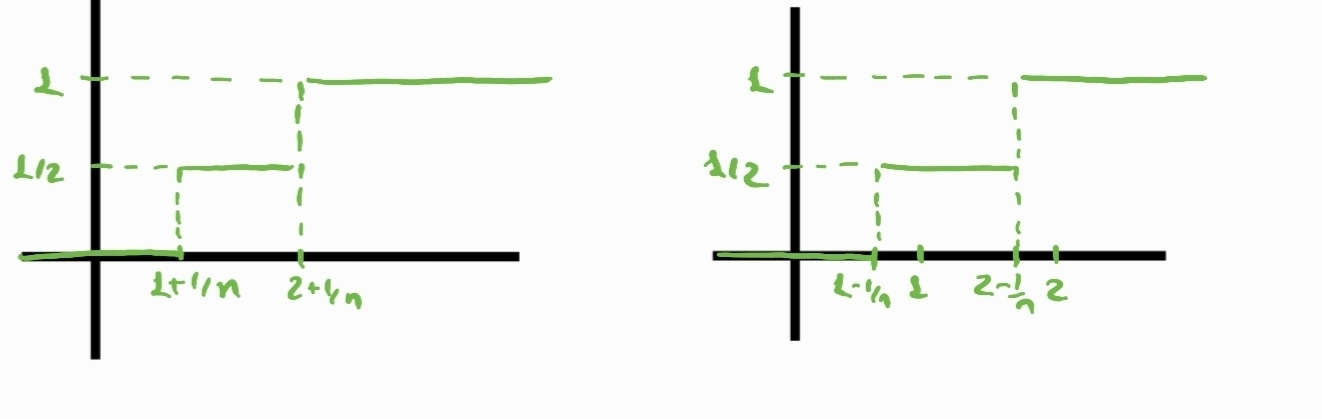
\includegraphics[scale=0.2]{6-1.jpg}
    \end{center}
    

    Notamos que:
    $$ \left\{
    \begin{array}{ll}
        x < 0 &  F_n(x) = 0 \to 0\\ 
        0<x<1 & \left\{
        \begin{array}{l}
            F_n(x) = 0\ n\ par\\ 
            \text{Si $ n $ impar y suf. grande, $ x<1-\dfrac{1}{n} $, por tanto }F_n(x) = 0
        \end{array}
        \right\} F_n(x) \to 0\\ 
        1<x<2 & \left\{
        \begin{array}{l}
            \text{Si $ n $ par y suf. grande, $ 1+\dfrac{1}{n}<x \implies F_n(x)=\dfrac{1}{2} $}\\
            \text{Si $ n $ impar, $ x<2-\dfrac{1}{2} $} \implies F_n(x)=\dfrac{1}{2}
        \end{array}
        \right\} F_n(x) \to \dfrac{1}{2}\\ 
        x>2 & \left\{
        \begin{array}{l}
            \text{Si $ n $ par y suf. grande, $ 2+\dfrac{1}{n}<x $} \implies F_n(x)=1\\ 
            \text{Si $ n $ impar,\ }F_n(x)=1
        \end{array}
        \right\} F_n(x) \to 1

    \end{array}
    \right. $$


    Por tanto, tenemos que:
    $$ F_n(x) \to F(x) = \left\{
    \begin{array}{ll}
        0 & x < 1 \\ 
        \dfrac{1}{2} & 1<x<2 \\ 
        1 & x>2
    \end{array}
    \right. $$

    Nos faltaría por definir el valor en 1 y 2. Para que $ F $ sea función de distribución hacemos que sea continua por la derecha:
$$F(x) = \left\{
    \begin{array}{ll}
        0 & x < 1 \\ 
        \dfrac{1}{2} & 1\leq x<2 \\ 
        1 & x\geq 2
    \end{array}
    \right. $$
    
\end{exercise}

\begin{exercise}
    Claramente tenemos que:
    $$ f(x)= \left\{
    \begin{array}{ll}
        \dfrac{1}{2} & x \in (0,2)\\ 
        0 & x \not \in (0,2)
    \end{array}
    \right. $$

    Entonces la función característica es:
    $$ \phi(t) = E(e^{itX_n}) = \int\limits_{0}^{2}e^{itx}\dfrac{1}{2}dx = \dfrac{1}{2} \dfrac{e^{itx}}{it} \Biggr|_{0}^{2} = \dfrac{e^{2it}-1}{2it} $$

    Por la independencia de los $ X_n $ tenemos que:
    $$ \phi_{Y_n}(t) = E(e^{itY_n}) = E(e^{itX_n})E(e^{it2X_{n+1}})E(e^{itX_{n+2}}) = \phi_n(t)\phi_{n+1}(2t)\phi_{n+2}(t) =$$ 
     $$ =  \left(\dfrac{e^{2it}-1}{2it}\right)^2 \dfrac{e^{2i2t}-1}{2i2t} = \dfrac{(e^{2it}-1)^2}{-4t^2} \dfrac{e^{4it}-1}{4it}$$

    Si $ Y_n-c $ es respecta respecto del origen, tenemos que $ E(Y_n-c)=0 \iff E(Y_n) = c $. Calculamos entonces $ E(Y_n) $:
    $$ c = E(Y_n) = E(X_n) +2(X_{n+1}) + E(X_{n+2}) = 1+2+1=4 $$

    Ya que $ E(X_n) = 1 $ (el punto medio del intervalo).

    Para comprobar si efectivamente $ Y_n-4 $ es simétrica, vemos si $ \phi_{Y_n-4}(t) $ es real:
    $$ \phi_{Y_n-4}(t) = E(e^{it(Y_n-4)}) = e^{-it4}E(itY_n) = e^{-it 4} \dfrac{(e^{2it-1}-1)}{2it} \dfrac{(e^{2it-1}-1)}{2it} \dfrac{e^{4it}-1}{4it} =$$ 
     $$ e^{-4it} e^{it} \dfrac{e^{it}-e^{-it}}{2it} e^{it}\dfrac{e^{it}-e^{-it}}{2it} e^{2it} \dfrac{e^{2it}-e^{-2it}}{4it}  = e^{-4it}e^{4it} \left( \dfrac{2i \sin(t)}{2it} \right)^2 \dfrac{2i \sin(2t)}{4it} = \dfrac{\sin^2(t)}{t^2} \dfrac{\sin(2t)}{2t} $$

    Luego sí es real y $ Y_n-4 $ es simétrica respecto del origen.

\end{exercise}

\begin{exercise}
    Consideramos las vvaa $ (X_i,Y_i,Z_i) $ donde:
    $$ X_i = \left\{
    \begin{array}{ll}
        1 & \text{si A gana el partido $ i$-ésimo}\\ 
        0 & \text{otro caso}
    \end{array}
    \right. $$
    $$ Y_i = \left\{
    \begin{array}{ll}
        1 & \text{si B gana el partido $ i$-ésimo}\\ 
        0 & \text{otro caso}
    \end{array}
    \right. $$
    $$ Z_i = \left\{
    \begin{array}{ll}
        1 & \text{si el partido $ i$-ésimo se empata}\\ 
        0 & \text{otro caso}
    \end{array}
    \right. $$
    Tenemos entonces que $ (X,Y,Z) = \sum\limits_{i=1}^{n}(X_i,Y_i,Z_i) $, que $ P((X_i,Y_i,Z_i)=(1,0,0)) = P((X_i,Y_i,Z_i)=(0,1,0)) = P((X_i,Y_i,Z_i)=(0,0,1)) = \dfrac{1}{3} $ y que son independientes las $ (X_i,Y_i,Z_i) $. Además:
    $$ f_i(t_1,t_2,t_3) = \dfrac{1}{3}(t_1+t_2+t_3) $$

    Por lo que $ f(t_1,t_2,t_3) $ vale:
    $$ f(t_1,t_2,t_3) = \left( \dfrac{1}{3}  \right)^{n} (t_1+t_2+t_3)^{n}  $$

    Utilizando la fórmula de Leibniz:

    $$ f(t_1,t_2,t_3) = \dfrac{1}{3^{n}} \sum\limits_{r_1+r_2+r_3=n}^{} \dfrac{n!}{r_1!r_2!r_3!} t_1^{r_1}t_2^{r_2}t_3^{r_3} $$

    Esta construcción corresponde a la distribución \textbf{multinomial}. La distribución que nos queda en base a $ f $ de $ (X,Y,Z)  $ es:
    $$ P((X,Y,Z)=(r_1,r_2,r_3)) = \dfrac{1}{3^{n}} \dfrac{n!}{r_1!r_2!r_3!} $$

    Con $ r_1+r_2+r_3=n $. enteros no negativos.

    Para el siguiente apartado usaremos que el dominio de $ f $ es todo $ \mathbb{R}^3 $, luego (1,1,1) es interior al dominio. Podemos ahora calcular las esperanzas que nos piden usando las derivadas parciales y evaluando en $ (1,1,1) $.

    $$ \dfrac{\partial f}{\partial t_1} = \dfrac{1}{3^{n}}n (t_1+t_2+t_3)^{n-1}  $$
    $$ \dfrac{\partial ^2f}{\partial t_1 \partial t_2} = \dfrac{1}{3^{n}}n(n-1) (t_1+t_2+t_3)^{n-2} $$
    $$ \dfrac{\partial ^3f}{\partial t_1 \partial t_2 \partial t_3} = \dfrac{1}{3^{n}}n(n-1)(n-2) (t_1+t_2+t_3)^{n-3} $$

    Evaluando en $ (1,1,1) $:
    $$ E(X) = \dfrac{\partial f}{\partial t_1}(1,1,1) = \dfrac{n}{3}  $$
    $$ E(XY) = \dfrac{\partial ^2 f}{\partial t_1 \partial t_2} (1,1,1) = \dfrac{n(n-1)}{3^2} $$
    $$ E(XY) = \dfrac{\partial ^3 f}{\partial t_1 \partial t_2 \partial t_3} (1,1,1) = \dfrac{n(n-1)(n-2)}{3^3} $$

\end{exercise}


\begin{exercise}
    Haciendo el cambio de variable quedaba al final que $$ g(u,v) = v e^{-v-u} $$ y las marginales quedaban que eran distribuciones Gamma. Se ve además que $ U,V $ son independientes, con lo que la función característica es el producto de las funciones característica de las marginales (que se pueden calcular con la integral Gamma). Para calcular la función característica de $ (X,Y) $ hacemos:
    $$ \phi_{(X,Y)}(t_1,t_2) = E(e^{i(t_1X+t_2Y)}) = E(e^{i(t_1(U+V))+t_2(U+2V)}) = E(e^{it_1U}e^{it_1V}e^{it_2U}e^{it_2 2V}) = $$ 
     $$=E(e^{(t_1+t_2)U}e^{i(t_1+2t_2)V})= \phi_{U}(t_1+t_2) \phi_{V}(t_1+2t_2) = \dfrac{1}{1-i(t_1+t_2)} \dfrac{1}{(1-i(t_1+2t_2))^2} $$ 

\end{exercise}



\chapter{Relación 7}

\begin{exercise}$  $
  \begin{flushright}
    \textbf{Apartado a)}
  \end{flushright}

  $$ F_n(x) = P(X_n\leq x) = \left\{
  \begin{array}{ll}
    0 & x<0\\ 
    \dfrac{1}{n} & 0\leq  x < a\\ 
    1 & x\geq a
  \end{array}
  \right. $$

  $$ \left\{
  \begin{array}{ll}
    F_n(x) = 0 \to 0 & x<0 \\ 
    F_n(x) = \dfrac{1}{n} \to 0 & 0<x<a \\ 
    F_n(x) = 1 \to 1 & x>a
  \end{array}
  \right. $$

  Estas funciones de distribución convergen entonces débilmente a la función

  $$ F(x) = \left\{
  \begin{array}{ll}
    0 & x<a \\ 
    1 & x>a
  \end{array}
  \right. $$
  
  Para que $ F $ sea una función de distribución, haremos que $ F(a) = 1 $. Nos preguntamos si hay convergencia en ese punto $ x=a $. Como $ F_n(a) = 1 $ siempre, sí hay convergencia en ese punto (aunque no nos haría falta al ser un punto de discontinuidad de $ F $). Por tanto, hemos llegado a que $ X_n $ converge en distribución a la v.a. de $ F $, es decir, la variable aleatoria $ X=a $ constante.


  \begin{flushright}
    \textbf{Apartado b)}
  \end{flushright}
  
  Para ver la convergencia en probabilidad, sabemos que si la hay, es ha $ X=a $ constante ya que tiene que coincidir con la convergencia en distribución. Además, sabemos que si $ X_n \to^{\mathcal{D}} a $, con $ a $ constante, entonces $ X_n \to^{P} a $

\begin{flushright}
    \textbf{Apartado c)}
\end{flushright}

Utilizaremos el Lema de Borel-Cantelli: si $ \sum\limits_{}^{}P(A_n) $ convergente $ \implies P(\limsup A_n) = 0 $ y si es divergente y los sucesos $ A_n $ son independientes, entonces $ P(\limsup A_n) = 1 $

Lo que nos piden es $ P(\limsup A_n) $ donde $ A_n = \{X_n = 0\} $. Además tenemos que $ P(A_n) = P(X_n  =0) = \dfrac{1}{n} \implies \sum\limits_{}^{}P(A_n) = \sum\limits_{}^{}\dfrac{1}{n} $ divergente. Además, los $ A_n $ son independientes, con lo que $ P(\limsup A_n) = P(X_n = 0,\ \text{infinitos valores de $ n $}) = 1 $

Para la segunda parte, sustituiríamos $ \dfrac{1}{n}  $ por $ \dfrac{n-1}{n} $, la cual también es divergente. Por tanto, la probabilidad buscada en este caso des de nuevo 0.

\begin{flushright}
    \textbf{Apartado d)}
\end{flushright}

Si convergiera, sería al límite en probabilidad (la variable aleatoria constante igual a $ a $). Usaremos que $ X_n $ converge casi seguramente si:
$$ \lim_{n \to \infty} P (\cap_{p\geq n} \{|X_{p}-a|<\varepsilon\}) = 1 $$

Observamos que:
$$ P(\cap_{p=n}^{\infty}\{|X_{p}-a|<\varepsilon\}) = \lim_{M \to \infty} P(\cap_{p=n}^{M}\{|X_{p}-a|<\varepsilon\}) =_{X_n\ indep} \lim_{M \to \infty} \prod_{p=n}^{M}P(|X_{p}-a|<\varepsilon) =_{Si\ \varepsilon<a}   $$
$$ = \lim_{M \to \infty} \prod_{p=n}^{M}\left(1-\dfrac{1}{p}\right) = \lim_{M \to \infty}\dfrac{n-1}{n} \dfrac{n-2}{n-1} \cdots \dfrac{M-1}{M} = \lim_{M \to \infty} \dfrac{n-1}{M} = 0  $$

Por tanto, $ X_n \cancel{\xrightarrow{cs}}\ a $

\begin{flushright}
    \textbf{Apartado e)}
\end{flushright}


Como la convergencia en media de orden $ p $ implica la convergencia en probabilidad tenemos que $ X_n $ solo tiene un candidato a límite en convergencia en media de orden $ p $, la v.a. constante $ a $. Buscamos entonces:
$$ E(|X_n-a|^{p}) \xrightarrow{n \to \infty} 0 $$


$$ |X_n-a|^{p} = \left\{
\begin{array}{ll}
    a^{p} & X_n = 0 \implies P(|X_n-a|^{p} = a^{p}) = P(X_n = 0) = \dfrac{1}{n}\\ 
    0 & X_n = a \implies P(|X_n-a|^{p}=0) = P(X_n = a) = \dfrac{n-1}{n}
\end{array}
\right. $$

Por tanto, $ E(|X_n-a|^{p}) = a^{p}\dfrac{1}{n} + 0 \dfrac{n-1}{n} = \dfrac{a^{p}}{n} \to 0 $, luego $ X_n \xrightarrow{m.a.p} a $


\begin{flushright}
    \textbf{Apartado f)}
\end{flushright}
Por la definición que tenemos de $ X_n $:
$$ E(X_n) = a \dfrac{n-1}{n} $$
$$ E(X_n^2) = a^2 \dfrac{n-1}{n} $$

Luego tenemos:
$$ Var(X_n) = a^2 \dfrac{n-1}{n}-a^2 \dfrac{(n-1)^2}{n^2} = a^2 \left( \dfrac{n(n-1)}{n^2} - \dfrac{(n-1)^2}{n^2} \right) = a^2 \dfrac{(n-1)}{n^2} $$
\begin{flushright}
    \textbf{Apartado g)}
\end{flushright}

Usaremos la regla de Stolz.

$$ \lim_{n \to \infty} \dfrac{E(S_n)}{n} = \dfrac{\sum\limits_{j=1}^{n}a \dfrac{j-1}{j}}{n} $$

Calculamos el siguiente límite, si existe el límite pedido y el calculado coincidirá:

$$\lim_{n \to \infty} \dfrac{E(S_n)-E(S_{n-1})}{n-(n-1)} = \lim_{n \to \infty} \dfrac{E(X_n)}{1} = \lim_{n \to \infty}a \dfrac{n-1}{n} = a$$

Entonces:
$$ \lim_{x \to \infty} \dfrac{E(S_n)}{n} = a $$

Haremos el mismo procedimiento para el otro límite:

$$ \lim_{n \to \infty} \dfrac{Var(S_n)-Var(S_{n-1})}{n^2-(n-1)^2} = \lim_{n \to \infty} \dfrac{Var(X_n)}{n^2-(n^2-2n+1)} = \lim_{n \to \infty} \dfrac{a^2 \dfrac{n-1}{n^2}}{2n-1} = 0$$

Por tanto:
$$ \lim_{n \to \infty} \dfrac{Var(S_n)}{n^2} = 0 $$


\begin{flushright}
    \textbf{Apartado h)}
\end{flushright}

Como $ \dfrac{Var(S_n)}{n^2}\to 0  $ entonces:
$$ \dfrac{S_n-E(S_n)}{n} \xrightarrow{P}0 $$

Además sabemos que $ \lim_{n \to \infty} \dfrac{E(S_n)}{n} = a $, por lo tanto tenemos que:
$$ \lim_{n \to \infty} \dfrac{S_n}{a} 0\ \text{ en probabilidad} $$

Y los $ a_n $ valen:
$$ a_n = E(S_n ) = \sum\limits_{j=1}^{n}a \dfrac{j-1}{j} $$

\end{exercise}

\newpage

\begin{exercise}
    $  $
    \begin{flushright}
        \textbf{Apartado a)}
    \end{flushright}
    
    
    Notamos que para $ x \in \left(0,\dfrac{1}{2}\right) $, $ x \in \left(0,\dfrac{1}{2}-\dfrac{1}{n}\right) $ para $ n $ suf. grande. Entonces $ X_n(x) =e^{-n}\to 0 $.
    
    En el caso $x \in  \left[\dfrac{1}{2},1\right)  $, $ x \in \left[\dfrac{1}{2},1-\dfrac{1}{n}\right) $ para $ n  $ suf. grande. Entonces $ X_n(x) = 1 \to 1 $.
    
    Por tanto, $ X_n $ converge casi seguramente a $ X $ con:
    $$ X(x) = \left\{
    \begin{array}{ll}
        0 & x \in \left(0,\dfrac{1}{2}\right)\\ 
        1 & x \in \left[\dfrac{1}{2},1\right)
    \end{array}
    \right. $$

    Ya que $ P(\lim_{n \to \infty}X_n = X) = P((0,1)) = 1 $

    Luego $ X_n $ también converge en probabilidad a $ X $.

    Notamos ahora que la función de distribución de $  X $ es:
    $$ F(x) = \left\{
    \begin{array}{ll}
        0 & x<0\\\\ 
        \dfrac{1}{2} & 0 \leq x < 1 \\\\ 
        1 & x>1
    \end{array}
    \right. $$

    \begin{flushright}
        \textbf{Apartado b)}
    \end{flushright}
    Como la convergencia en media de orden $ p $ implica la convergencia en probabilidad tenemos que $ X_n $ solo puede converger en media de orden $ p $ a $ X $ (o a otra casi seguramente igual).

    Notamos en primer lugar que $ E(|X_n|^{p}) <+\infty $ y $ E(|X|^{p}) <+\infty $. Calculamos ahora la esperanza de $ |X_n-X|^{p} $
    $$ E(|X_n-X|^{p}) = |e^{-n}-0|^{p}\cdot \left(\dfrac{1}{2}-\dfrac{1}{n}\right)+|1-0|^{p} \dfrac{1}{n} + |1-1|^{p}\left(\dfrac{1}{2}-\dfrac{1}{n}\right) + |e^{n}-1|^{p} \dfrac{1}{n} = $$ 
    $$ =  e^{-np}\left(\dfrac{1}{2}-\dfrac{1}{n}\right) +\dfrac{1}{n}+(e^{n}-1)^{p}\dfrac{1}{n} \to \infty  $$

    Por tanto, no hay convergencia en media de orden $ p $

    \begin{flushright}
        \textbf{Apartado c)}
    \end{flushright}
    Escribimos primero $ F_n $ la función de distribución de $ X_n $:
    $$ F_n(x) = \left\{
    \begin{array}{ll}
        0 & x<e^{-n}\\ \\ 
        \dfrac{1}{2}-\dfrac{1}{n} & e^{-n}\leq  x <1\\\\ 
        1-\dfrac{1}{n} & 1\leq x<e^{n}\\\\ 
        1 & e^{n}\leq  x 
    \end{array}
    \right. $$

    Estudiaremos la convergencia punto a punto de las $ F_n $. $ F_n $ converge a:
    $$G(x) =  \left\{
    \begin{array}{ll}
        0 & x\leq  0\\ \\
        \dfrac{1}{2} & 0<x<1\\ \\
        1 & x\geq 1

    \end{array}
    \right. $$

    Entonces tenemos que $ F_n\xrightarrow{d}G $ pero no podemos hablar de convergencia en distribución aún ya que $ G $ no es continua por la derecha. Tenemos que modificar $ G $ para que sea una función de distribución. El cambio obvio nos da la $ F $ que vimos previamente, la que es la función de distribución de $ X $. Por tanto $ X_n \xrightarrow{\mathcal{D}}X $.

    Notemos que la modificación que hacemos en $ G $ no importa para la convergencia débil de $ F_n $ ya que el punto que cambiamos no pertenece a $Cont\ G $


    \textbf{Observación}

    Podemos definir variables aleatorias que converjan en distribución a $ X $. Haremos que sus funciones de distribución coincidan con $ F $:

    $$ Y_n(x) = \left\{
    \begin{array}{ll}
        0 & \dfrac{1}{2} <x<1 \\ \\ 
        1 & 0 \leq x < \dfrac{1}{2}
    \end{array}
    \right. $$

    $$ Z_n(x) = \left\{
    \begin{array}{ll}
        0 & x \in \left(\dfrac{1}{4},\dfrac{2}{4}\right) \cup \left(\dfrac{3}{4},1\right)\\ \\ 
        1 & x \in \left(0,\dfrac{1}{4}\right) \cup \left(\dfrac{2}{3},\dfrac{3}{4}\right)\\ \\ 
        17 & x \in \left\{\dfrac{1}{4},\dfrac{2}{4},\dfrac{3}{4}\right\}
    \end{array}
    \right. $$

\end{exercise}


\chapter{Relación 8}

\begin{exercise}
    $  $

    Recordemos que decimos que $ X_n\xrightarrow[]{P}X $ si $ P(|X_n-X|<\varepsilon) \to 1 \forall \varepsilon>0 $ o bien $ P(|X_n-X|>\varepsilon) \to 0 \forall \varepsilon>0 $. Como no sabemos muy bien qué $ X $ tomar, tratar de buscar el límite en distribución de $ X_n $. Entonces podríamos tomar $ X $ como ese límite. Si no existiera convergencia en distribución, ya sabríamos que no existe convergencia en probabilidad.

    Para obtener entonces la convergencia en distribución, necesitamos las distribuciones de las $ X_n $:
    $$ P(X_n = 0) = P((-\infty,\dfrac{1}{n})) = \int\limits_{-\infty}^{1/n}f(t)dt = \int\limits_{0}^{1/n} \lambda e^{-\lambda t}dt = -e^{-\lambda t} \Biggr|_{0}^{1/n} = -e^{-\lambda/n}+1 = 1-e^{-\lambda/n}$$
    $$ P(X_n = 3) = P\left(\left\{\dfrac{1}{n}\right\}\right) = 0 $$
    $$ P(X_n = 1) = P\left(\left(\dfrac{1}{n},n\right]\right) = \int\limits_{1/n}^{n} \lambda e^{-\lambda t}dt = -e^{-\lambda t} \Biggr|_{1/n}^{n} = e^{-\lambda/n} - e^{-\lambda n} $$
    $$ P(X_n = e^{n \lambda}) = e^{-n \lambda} $$

    Luego la función de distribución de $ X_n $ es:
    $$ F_n(x) = \left\{
    \begin{array}{ll}
        0 & x < 0 \\ 
        1-e^{-\lambda/n} & 0\leq  x< 1\\ 
        1-e^{-n \lambda} & 1\leq  x< e^{n \lambda}\\ 
        1 & x \geq  e^{n \lambda}
    \end{array}
    \right. $$
    
    Si $ \lambda $ es muy pequeño, los primeros valores de $ n $ no estarán ordenados así exactamente, pero a partir de cierto $ n $, $ e^{n\lambda} > 1 $ y no tendríamos problemas. Vemos la convergencia ahora de $ F_n $:
    $$ \left\{
    \begin{array}{ll}
        
        F_n(x) = 0 \to 0 & x<0 \\ 
        F_n(x) = 1-e^{-\lambda/n} \to 0 & 0<x<1 \\ 
        F_n(x) = 1-e^{-n \lambda} \to 1 & x>1\\ 
    \end{array}
    \right. $$

    Entonces 
    $$ F_n(x) \to F(x) = \left\{
    \begin{array}{ll}
        0 & x<1 \\ 
        1 & x\geq  1
    \end{array}
    \right. \implies X = 1 c.s. $$
    
    Como $ X = d $ con $ d $ constante y $ X_n \xrightarrow[]{\mathcal{D}} X = 1 $, entonces $ X_n \xrightarrow[]{P} X=1 $.

    Vamos ahora con la convergencia de orden 2. Como $ X $ converge en probabilidad, si $ X_n $ tiene convergencia en media de orden 2, entonces es a $ X $. Calculamos las siguientes esperanzas para ver si tienden a cero cuando $ n\to\infty $:
    $$ E(|X_n-1|^2) = (0-1)^2 (1-e^{-\lambda/n})+(3-1)^2\cdot 0 + (1-1)^2\cdot (...) + (e^{n\lambda}-1)^2 e^{-\lambda n} = $$ 
    $$=1(1-e^{-\lambda/n}) + (e^{n\lambda}-1)^2e^{-\lambda n} = 1-e^{-\lambda/n} +(e^{2n\lambda}-2e^{n\lambda}+1)e^{-n\lambda} = $$
    $$ = 1-e^{-\lambda/n} + e^{n\lambda}-2+e^{-n\lambda} \cancel{\to} 0 $$

    Luego no hay convergencia cuadrática.
\end{exercise}

\begin{exercise}
    $  $

    \begin{flushright}
        \textbf{Apartado a)}
    \end{flushright}
    

    Recordemos primero que los límites en probabilidad a una constante son equivalentes a los límites en distribución.

    Para abordar este teorema, expresaremos $ X_n $ de forma más compacta, aprovechando la aleatoriedad de su definición. Para ello, definimos una variable aleatoria $ Z_n $ que represente lo que obtenemos al lanzar la moneda.

    $$ Z_n = \left\{
    \begin{array}{ll}
        0 & \text{si cara en $ n $-ésimo lanzamiento}\\ 
        1 & \text{si cruz en $ n $-ésimo lanzamiento}\\ 
    \end{array}
    \right. $$

    Entonces tenemos:
    $$ X_n = Y_n+Z_nY_{n+1} $$

    Sabemos además que las vvaa $ Y_n,Z_m $ son independientes. Haremos los cálculos necesarios para obtener $ E(S_n)$:

    $$ E(Y_n) = \int\limits_{0}^{2} y\cdot \dfrac{1}{2}dy = \dfrac{1}{2} \dfrac{y^2}{2} \Biggr|_{0}^{2} = 1 $$
    $$ E(Z_n) = 0\cdot \dfrac{1}{2} + 1\cdot \dfrac{1}{2} = \dfrac{1}{2} $$
    $$ E(Y_n^2) = \int\limits_{0}^{2}y^2\dfrac{1}{2}dy = \dfrac{1}{2} \dfrac{y^3}{3} \Biggr|_{0}^{2} = \dfrac{4}{3} $$
    $$ E(Z_n^2) = \dfrac{1}{2} $$
    $$ E(X_{n}) = E(X_n+Z_nY_{n+1}) = E(Y_n)+E(Z_n)E(Y_{n+1}) = 1+\dfrac{1}{2} = \dfrac{3}{2} $$


    Finalmente llegamos a:
    $$ E(S_n) = E\left(\sum\limits_{r=1}^{n}X_{r}\right) = \sum\limits_{r=1}^{n}E(X_{r}) = \dfrac{3}{2}n $$

    Tenemos que calcular ahora $ Var(S_n) $:
    $$ Var(S_n) = \sum\limits_{r=1}^{n}Var(X_{r}) +2 \sum\limits_{r<s}^{}Cov(X_{r},X_{s}) $$

    Entonces tenemos
    $$ Var(X_n) = Var(Y_n+Z_nY_{n+1}) = Var(Y_n)+Var(Z_nY_{n+1}) +\cancelto{0}{2Cov(Y_n,Z_nY_{n+1})} $$
    $$ Var(Y_n) = E(Y_n^2)-(E(Y_n))^2 = \dfrac{4}{3}-1 = \dfrac{1}{3}$$
    $$ Var(Z_nY_{n+1}) = E(Z_n^2Y_{n+1}^2)-E(Z_nY_{n+1})^2 = \dfrac{1}{2}\dfrac{4}{3}-\left(\dfrac{1}{2}\cdot 1\right)^2 = \dfrac{2}{3}-\dfrac{1}{4} = \dfrac{5}{12} $$

    Luego $ Var(X_n) $ vale:
    $$ Var(X_n) = \dfrac{1}{3}+\dfrac{5}{12} = \dfrac{3}{4} $$

    Nos falta calcular $ Cov(X_{r},X_{s}) $

    $$ Cov(X_{r},X_{s}) = Cov(Y_{r}+Z_{r}Y_{r+1},Y_{s}+Z_{s}Y_{s+1}) $$

    Podríamos pensar que se va a anular siempre por la independencia, pero nos tendremos que detener en el caso $ r=s-1 $ ya que en ese caso tendremos $ (Y_{s-1}+Z_{s-1}Y_{s},Y_{s}+Z_{s}Y_{s+1}) $ y no son independientes (en principio).

    Por tanto, el sumatorio $ \sum\limits_{r<s}^{}Cov(X_{r},X_{s}) $ lo podemos cambiar por $ \sum\limits_{s=1}^{n}Cov(X_{s},X_{s+1}) $. Vamos a calcular esas covarianzas.

    $$ Cov(X_{s},X_{s+1}) = Cov(Y_{s}+Z_{s}Y_{s+1},Y_{s+1}+Z_{s+1}Y_{s+2}) =\footnote{La covarianza es bilineal}$$ 
    $$ =\cancel{Cov(Y_{s},Y_{s+1})} + \cancel{Cov(Y_{s},Z_{s+1}Y_{s+2})} + Cov(Z_{s}Y_{s+1},Y_{s+1}) + \cancel{Cov(Z_{s}Y_{s+1},Z_{s+1}Y_{s+2})} =$$ 
    $$= E(Z_{s}Y_{s+1}^2)-E(Z_{s}Y_{s+1})E(Y_{s+1}) = E(Z_{s})E(Y_{s+1}^2)-E(Z_{s})E(Y_{s+1}^2) = \dfrac{1}{2}\dfrac{4}{3}-\dfrac{1}{2}1 = \dfrac{1}{6}$$

    Podemos finalmente calcular $ Var(S_n) $:
    $$ Var(S_n) = \dfrac{3}{4}n +2 \dfrac{1}{6}(n-1) = \dfrac{13n-4}{12} $$

    \begin{flushright}
        \textbf{Apartado b)}
    \end{flushright}

    Como tenemos:
    $$ \dfrac{Var(S_n)}{n^2} = \dfrac{\dfrac{13n-4}{12}}{n^2} \to 0 $$

    Entonces tenemos un teorema que nos dice que $ \dfrac{S_n-E(S_n)}{n}\xrightarrow[]{P}0 $ y que si $ \dfrac{E(S_n)}{n} $ converge, entonces $ \dfrac{S_n}{n} $ converge a lo mismo. Es fácil ver que:

    $$ \dfrac{E(S_n)}{n}\to \dfrac{3}{2} $$

\end{exercise}

\begin{exercise}
    Al ser las $ X_n $ suma de normales, las $ X_n $ son normales. La media de la $ X_n $ es claramente $ 2\mu +\mu +2\mu = 5\mu $. Además, como las $ Y_n $ son independientes, la varianza de las $ X_n $ es $ 4\rho ^2 $.

    Vamos a trabajar ahora con las $ S_n $, observamos en primer lugar que:
    $$ S_n = \sum\limits_{r=1}^{n}X_{r} = \sum\limits_{r=1}^{n} (Y_{2r-1}+Y_{2r}+Y_{2r+1}) = \sum\limits_{r=1}^{n}Y_{2r-1}+ \sum\limits_{r=1}^{n}Y_{2r}+\sum\limits_{r=1}^{n}Y_{2r+1} = $$ 
    $$ = Y_1 + \sum\limits_{r=2}^{n} Y_{2r-1} + \sum\limits_{r=1}^{n}Y_{2r} + \sum\limits_{r=1}^{n-1}Y_{2r+1} + Y_{2n+1} = Y_1+ 2 \sum\limits_{r=1}^{n-1} Y_{2r+1} + \sum\limits_{r=1}^{n}Y_{2r} + Y_{2n+1} =$$
    $$ =  Y_1+ \sum\limits_{r=1}^{n-1} 2Y_{2r+1} + \sum\limits_{r=1}^{n}Y_{2r} + Y_{2n+1}$$

    Luego los $ S_n $ son sumas de normales independientes. Buscaremos su media y su varianza (recordemos que $ Var(aX) = a^2Var(X) $).

    $$ E(S_n) = 2\mu +2\mu +(n-1)2\cdot 2\mu + n\mu = 5n\mu $$
    $$ Var(S_n) = 2\sigma ^2 +2\sigma ^2 +(n-1)2^2\cdot 2\sigma ^2+n\sigma ^2 =  (9n-4)\sigma ^2$$

    Otra forma para de calcular $ Var(S_n) $ sería la siguiente:
    $$ Var(S_n) = \sum\limits_{r=1}^{n}Var(X_{r})+2 \sum\limits_{r<s}^{}Cov(X_{r},X_{s}) $$

    Entonces veríamos que:
    $$ Cov(X_{r},X_{s}) = \left\{
    \begin{array}{ll}
        0 & s \ne r+1\\ 
        Cov(X_{r}X_{r+1}) & s = r+1
    \end{array}
    \right. $$

    Luego podríamos reescribir $ Var(S_n) $ como:
    $$ Var(S_n) = \sum\limits_{r=1}^{n}Var(X_{r})+2 \sum\limits_{r=1}^{n-1}Cov(X_{r},X_{r+1}) $$

    $$ Cov(X_{r},X_{r+1}) = Cov(Y_{2r+1}+Y_{2r}+Y_{2r+1},Y_{2r+1}+Y_{2r+2}+Y_{2r+3}) =\footnote{Por la bilinealidad de $ Cov $} Cov(Y_{2r+1},Y_{2r+1}) = $$ 
    $$=Var(Y_{2r+1}) = 2\sigma ^2 $$

    Luego finalmente:

    $$ Var(S_n) = n\cdot 5\cdot \sigma ^2 + 2(n-1)2\sigma ^2 = (9n-4)\sigma ^2 $$

    Volviendo a lo que nos pedía el problema, sabemos que:
    $$ \dfrac{S_n-E(S_n)}{\sqrt{Var(S_n)}} = \dfrac{S_n-5n\mu}{\sqrt{9n-4}\sigma} \sim \mathcal{N}(0,1) $$

    Luego esa sucesión converge en distribución a $ \mathcal{N}(0,1) $.


\end{exercise}



\chapter{Relación 9}

\begin{exercise}
    $  $
    \begin{flushright}
        \textbf{Apartado a)}
    \end{flushright}

    \begin{flushright}
        \textbf{Apartado b)}
    \end{flushright}
    
    Veremos que en este caso $ Z_n $ no es una cadena de Markov. Comprobaremos que para un $ (k,j)  $ concreto, no se da la igualdad:
    $$ P_{kj} = P(Z_n = j|Z_0 = 0,Z_1=j_1,...,Z_{n-1} = k) = P(Z_n=j|Z_{n-1} = k) $$

    Observamos que:
    $$ P(Z_m = 0 |Z_{m-1} = 0) = P(Z_m = 0| X_{m-1} = 1,X_{m-2} = 0) = p $$
    $$ P(Z_m = 1 | Z_{m-1} = 0) = 1-P(Z_m = 0 |Z_{m-1} = 0) = 1-p = q $$

    $$ P(Z_m = 0|Z_{m-1} = 1) = P(Z_m = 0|\{X_{m-1} = 0,X_{m-2} = 1\} \cup \{X_{m-1} = 1,X_{m-2} = 0\}\cup $$  
    $$\cup \{X_{m-1}=0\cup X_{m-2} = 0\}) = $$  
    $$\dfrac{P(\{X_{m-1} = 1,X_m = 1\}\cap \{X_{m-1} = 0,X_{m-2} = 1\ \acute o\ X_{m-1} = 1,X_{m-2} = 0\ \acute o\ X_{m-1} = 0,X_{m-2} = 0\})}{P(\{X_{m-1}=1,X_{m-2}=0\}\cup\{X_{m-1}=0,X_{m-2}=1\}\cup \{X_{m-1}=0,X_{m-2}=0\})} $$

    $$ = \dfrac{P(\emptyset)+P(\{X_{m-2}=0,X_{m-1}=1,X_{m}=1\}) + P(\emptyset)}{P(\{X_{m-1} = 1,X_{m-2} =1\}^{c})} = \dfrac{qp^2}{1-p^2} = \dfrac{\cancel{q}p^2}{\cancel{(1-p)}(1+p)}$$
    
    Entonces vemos que:
    $$ P(Z_m = 0|Z_{m-1} = 0,Z_{m-2} = 0) = $$  
    $$=  P\left(X_{m-1}=1,X_m = 1 \Biggr| \left\{
    \begin{array}{cc}
        X_{m-1} & X_{m-2}\\0 & 1\\ 1 & 0 \\ 0 & 0
    \end{array}
    \right\},X_{m-2} = 1,X_{m_3} = 1\right) =$$ 
    $$=P(X_{m-1} = 0,X_{m}=1|X_{m-1} = 0,X_{m-2} = 1,X_{m-3} = 1) = 0 \ne \dfrac{p^2}{1+p} $$

    Donde las llaves representan los posibles valores que pueden tomar $ (X_{m-1},X_{m-2}) $ para que $ Z_{m-1} = 0 $

    
\end{exercise}

\begin{exercise}
    $  $

    Observamos primero que $ X_n $ puede tomar los valores $ \{0,1,2,3,4,5,6\} $. Obtenemos los valores:
    $$ P_{00} = \dfrac{1}{6} $$
    
    Los resultados de los dados en este caso son $ (1,j),(1,j') $
    $$ P_{01} = \dfrac{5}{6}\dfrac{1}{6} $$

    Para este caso tendremos $ (1,j),(i\ne 1,2) $. Análogamente tendremos:
    $$ P_{02} = \dfrac{5}{6}\dfrac{1}{6} \dots\ P_{06}= \dfrac{5}{6}\dfrac{1}{6} $$

    Calcularemos ahora $ P_{10} $, la secuencia de valores obtenidos ha de ser $ (i\ne 1,1),(1,j) $:
    $$ P_{10}  = \dfrac{1}{6} $$

    Para $ P_{11} $ tendremos $ (i\ne 1,1),(i\ne 1,1) $ y de forma análoga obtenemos $ P_{1n} $:
    $$ P_{11} = P_{12} = ... = P_{16} = \dfrac{5}{6}\dfrac{1}{6} $$

    Supongamos que estamos ahora en el estado 2. Por tanto, tenemos una sucesión de valores que comienza con una tirada de la forma $ (1,j) $ a la que sigue una secuencia de tiradas de la forma $ (i\ne 1,j') $ con $ j' = 1,2 $. Alguno de estos $ j' $ toma el valor 2. 

    Para el estado $ P_{20} $, sabemos directamente que $ P_{20} = \dfrac{1}{6} $.
    
    Por otro lado, $ P_{21} = 0 $ ya que en las tiradas anteriores ya hemos conseguido al menos un 2 en el dado rojo (y ninguno mayor). Por tanto, aunque obtengamos un 1 en el dado rojo ahora, seguiremos en el estado 2.
    
    De forma parecida, obtenemos que $ P_{22} $ es la probabilidad de no sacar un 1 en el dado negro y la de sacar un 1 o un 2 en el estado rojo en la próxima tirada. En definitiva, $ P_{22} = \dfrac{5}{6}\dfrac{2}{6} $.

    Por último, $ P_{2j} $ para $ j \geq  3 $ tendremos que hacer una tirada de la forma $ (i\ne 1,j) $, luego $ P_{23} = ... = P_{26} = \dfrac{5}{6}\dfrac{1}{6} $

    Supongamos ahora que estamos en el estado 3, con los mismo razonamientos que en el caso anterior, podemos obtener los siguientes valores:
    $$ 
    \begin{matrix}
        P_{20} = \dfrac{1}{6} & P_{31} = 0 & P_{32} = 0 & P_{33} = \dfrac{5}{6}\dfrac{3}{6} & P_{34} = \dfrac{5}{6}\dfrac{1}{6}  & P_{35} = \dfrac{5}{6}\dfrac{1}{6} & P_{36} = \dfrac{5}{6}\dfrac{1}{6}
    \end{matrix}
    $$ 

    Es una cadena de Markov porque solo dependemos del estado anterior para pasar al siguiente.

    Entones la matriz de probabilidades de transición sería:
    $$
    \begin{pmatrix} 
    \dfrac{1}{6} & \dfrac{5}{6}\dfrac{1}{6} & \dfrac{5}{6}\dfrac{1}{6} & \dfrac{5}{6}\dfrac{1}{6}& \dfrac{5}{6}\dfrac{1}{6}& \dfrac{5}{6}\dfrac{1}{6} & \dfrac{5}{6}\dfrac{1}{6}\\ \\
    \dfrac{1}{6} & \dfrac{5}{6}\dfrac{1}{6} & \dfrac{5}{6}\dfrac{1}{6} & \dfrac{5}{6}\dfrac{1}{6} & \dfrac{5}{6}\dfrac{1}{6} & \dfrac{5}{6}\dfrac{1}{6} & \dfrac{5}{6}\dfrac{1}{6} \\ \\
    \dfrac{1}{6} & 0 & \dfrac{5}{6}\dfrac{2}{6} & \dfrac{5}{6}\dfrac{1}{6} & \dfrac{5}{6}\dfrac{1}{6} & \dfrac{5}{6}\dfrac{1}{6} & \dfrac{5}{6}\dfrac{1}{6}\\ \\ 
    \dfrac{1}{6} & 0 & 0 & \dfrac{5}{6}\dfrac{3}{6} & \dfrac{5}{6}\dfrac{1}{6} & \dfrac{5}{6}\dfrac{1}{6} & \dfrac{5}{6}\dfrac{1}{6} \\ \\
    \dfrac{1}{6} & 0 & 0 & 0 & \dfrac{5}{6}\dfrac{4}{6} & \dfrac{5}{6}\dfrac{1}{6} & \dfrac{5}{6}\dfrac{1}{6}\\ \\ 
    \dfrac{1}{6} & 0 & 0 & 0 & 0 & \dfrac{5}{6} \dfrac{5}{6} & \dfrac{5}{6}\dfrac{1}{6} \\ \\ 
    \dfrac{1}{6} & 0 & 0 & 0 & 0 & 0 & \dfrac{5}{6}
    \end{pmatrix}  $$
    
    \begin{flushright}
    \textbf{Apartado extra)}
\end{flushright}

\textbf{Obtener la matriz de probabilidades iniciales en los siguientes casos:}

\begin{flushright}
    \textbf{Apartado a)}
\end{flushright}
El estado inicial de la cadena lo determina el valor obtenido en un dado en un lanzamiento cero.

$$ a = \left[ 0 \ \dfrac{1}{6} \ \dfrac{1}{6} \ \dfrac{1}{6} \ \dfrac{1}{6} \ \dfrac{1}{6} \ \dfrac{1}{6} \right] $$

\begin{flushright}
    \textbf{Apartado b)}
\end{flushright}
El estado inicial se determina de forma totalmente aleatoria:
$$ a = \left[ \dfrac{1}{7} \ \dfrac{1}{7} \ \dfrac{1}{7} \ \dfrac{1}{7} \ \dfrac{1}{7} \ \dfrac{1}{7} \ \dfrac{1}{7} \right] $$


\begin{flushright}
    \textbf{Apartado c)}
\end{flushright}

El estado inicial se determina en un lanzamiento cero de un dado siendo 0 si en el dado se obtiene 1 y 1 en caso contrario.
$$ a = \left[\dfrac{1}{6}\ \dfrac{5}{6}\ 0\ 0\ 0\ 0\ 0\right] $$


\end{exercise}

\begin{exercise}
    \textbf{Ejercicio extra}

    Supongamos que tenemos una cadena de Markov que representa un movimiento aleatorio sobre los puntos de la recta de coordenadas:
    
    $$S = \{...,-2,-1,0,1,2,3,4,...\} $$

    Siendo las probabilidades de transición:
    $$ 
    \begin{matrix}
        P_{jj+1} = p & P_{jj-1} = q = 1-p  
    \end{matrix}$$

    Buscaremos los estados de no retorno, de retorno, transitorios y persistentes. Recordemos que:
    $$ \left\{
    \begin{array}{ccc}
        \text{de no retorno} &  f_{jj} = 0 \iff P_{jj}^{n} = 0 & \forall  n \geq  1      \\ 
        \text{de retorno} &  f_{jj} > 0 \iff P_{jj}^{n} > 0 & \text{algún}  n \geq  1 \\ 
        \text{transitorio} &  f_{jj} < 1 \iff \sum\limits_{}^{} P_{jj}^{n}  & \text{convergente}\\ 
        \text{persistente} &  f_{jj} = 1 \iff \sum\limits_{}^{} P_{jj}^{n}  & \text{divergente}
    \end{array}
    \right\} $$

    Usaremos también la fórmula de Stirling 
    $$ \lim_{n \to \infty} \dfrac{n! }{n^{n}e^{-n}\sqrt{2\pi n}} = 1 \iff n ! \sim n^{n}e^{-n} \sqrt{2\pi n} $$


    Calcularemos ahora los $ P_{jj}^{n} $
    $$ P_{jj}^{n} = \sum\limits_{}^{} P_{jk_1}P_{k_1k_2}\cdots P_{k_nj} $$

    Como si avanzamos $ m $ posiciones, tendremos que retroceder otras $ m $, necesitaremos que $ n $ sea par para que la probabilidad sea no nula:
    $$ P_{jj}^{n} = 0\ \forall n \ne 2m $$
    $$ P_{jj}^{2m} = \sum\limits_{}^{} p^{m}q^{m} $$

    El número de sumandos serán las formas de ordenar los pasos a derecha e izquierda, es decir, $ \binom{2m}{m} $. Por tanto:
    $$ P_{jj}^{2m} = \binom{2m}{m}p^{m}(1-p)^{m} $$

    Por tanto, en el caso de que $ p = 0,1 $, todos los estados son de no retorno.

    En el resto de casos, los estados serán de retorno.

    Tendremos que estudiar ahora la convergencia de la serie usando la fórmula de Stirling:
    $$ \sum P_{jj}^{2m} = \sum\limits_{m=1}^{\infty} \dfrac{(2m)!}{m!m!}p^{m}(1-p)^{m}  = \sum\limits_{m=1}^{\infty} \dfrac{(2m)^{2m}e^{-2m}\sqrt{2\pi 2m}}{m^{2m}e^{-2m}2\pi m}p ^{m}(1-p)^{m} =$$
    $$ = \sum\limits_{m=1}^{\infty} \dfrac{2^{2m}2 \sqrt{\pi m}}{2 \pi m} p^{m}(1-p)^{m}= \sum\limits_{m=1}^{\infty} \dfrac{4^{m}}{\sqrt{\pi m}} p^{m}q^{m} =$$
    $$  = \sum \dfrac{(4pq)^{m}}{\sqrt{\pi m}} \leq  \sum\limits_{}^{} (4pq)^{m} $$

    Usando que $ f(p) = p(1-p) $ es una parábola con máximo en $ p=\dfrac{1}{2} $ con valor $ f\left(\dfrac{1}{2}\right) = \dfrac{1}{4} $ y que se anula en $ p=0,1 $, tenemos que la serie converge cuando $ p \ne \dfrac{1}{2} $ (serie geométrica de razón menor que 1). En ese caso los estados son transitorios.

    En el caso $ p = \dfrac{1}{2} $ tendremos que la serie es de la forma $ \sum\limits_{}^{} \dfrac{1}{m^{1/2}} $, que es divergente. Por lo tanto, en este caso todos los estados son persistentes.


\end{exercise}

\end{document}
                


% Esto no se si es importante lo copio aqui fuera


% Un expermiento se puede repetir un gran numero de veecs en condiciones similares pudiendo obtener como resultado $ A $ o su complementario

% $$ \Epsilon_1,...,\Epsilon_n $$

% Frecuenica absoluta de $ A $ a lo largo de los $ n $ experimentos $ n_{A} $: $ fr(A,n) = \dfrac{n_{A}}{n} $

% La frencuencia relativa de $ A $ se basa en la ley de regularidad de frecuencias:

% La frecuencia relativa de un suceso $ A $ se aproxima a un valor cuando el numero de repeticiones es grande. A este valor le llamamos probabilidad de $ A $.

% $$ X_j = \left\{
% \begin{array}{ll}
%     1 & \text{si en el experimento j-ésimo se obiene }A\\ 
%     0 & \text{si en el experimento j-ésimo no se obiene }A\\ 
% \end{array}
% \right. $$

% $ X_j \sim $ Bernoulli de parametros $ P(X_j=1)=p=P(A) $ independientes.

% $$ S_n = X_1+X_2+...+X_n $$ representa 

% $$ \dfrac{S_n}{n} \xrightarrow{P} \mu = p = P(A) $$
% $$ \dfrac{n_{A}}{n} \xrightarrow{P} \mu  = P(A) $$

% No sé qué es esto. Creo que es una anotacion de la ultima demo de la parte de ley debil

% Sea $ f $ una función derivable en el origen, entonces $ f'(0)=0 $:
% $$ \lim_{h \to 0} \dfrac{f(0+h)-f(0)}{h} = \left\{
% \begin{array}{l}
%     \lim _{\substack{h \to 0\\ h>0}}} \dfrac{f(0+h)-f(0)}{h} =  \lim_{h \to 0} \dfrac{f(h)-f(0)}{h} = L_1\\ 
%     \lim _{\substack{h \to 0\\ h<0}}} \dfrac{f(0+h)-f(0)}{h} =  \lim_{h \to 0} -\dfrac{f(-h)-f(0)}{-h} = \lim_{h \to 0} \dfrac{f(-h)-f(0)}{-h} = -L_1\\ 

    
% \end{array}
% \right. \implies L_1=-L_1 \implies L_1 = 0$$


% Comentario de la definicion de ley fuerte

$$ \left\{
\begin{array}{l}
    \dfrac{S_n-a_n}{n} \xrightarrow{cs}a\\ 
    \dfrac{a_n}{n} \to a
\end{array}
\right.\implies \dfrac{S_n}{n} \to a $$

Además:

$$ \left\{
\begin{array}{l}
    \dfrac{S_n}{n} \to a\\ 
    \dfrac{a_n}{n} \to a
\end{array}
\right. \implies \dfrac{S_n-a_n}{n} \xrightarrow{cs}a$$


%Un par de teoremas enunciados antes del primer teorema de ley fuerte. (El teorema nos da ambos resultados)

\begin{theorem}
    Teorema de Borel

    $ X_1,X_2,... $ independientes Bernoulli de parámetro $ p $, $ S_n = X_1+X_2+...+X_n $

    $$ \lim_{n \to \infty} P(\bigcap_{r\geq n} \{|\dfrac{S_{r}}{p}|<\varepsilon\}) = 1\hspace{5mm} \forall \varepsilon>0 $$
\end{theorem}


\begin{proposition}
    Condición necesaria y suficiente para que $ X_n\xrightarrow{cs}X  $
    $$ \lim_{n \to \infty}P( \{\cap_{p\geq n}|X_{p}-X|<\varepsilon\}) = 1 \hspace{5mm} \forall \varepsilon>0 $$
\end{proposition}